%% abtex2-modelo-trabalho-academico.tex, v-1.9.6 laurocesar
%% Copyright 2012-2016 by abnTeX2 group at http://www.abntex.net.br/ 
%%
%% This work may be distributed and/or modified under the
%% conditions of the LaTeX Project Public License, either version 1.3
%% of this license or (at your option) any later version.
%% The latest version of this license is in
%%   http://www.latex-project.org/lppl.txt
%% and version 1.3 or later is part of all distributions of LaTeX
%% version 2005/12/01 or later.
%%
%% This work has the LPPL maintenance status `maintained'.
%% 
%% The Current Maintainer of this work is the abnTeX2 team, led
%% by Lauro César Araujo. Further information are available on 
%% http://www.abntex.net.br/
%%
%% This work consists of the files abntex2-modelo-trabalho-academico.tex,
%% abntex2-modelo-include-comandos and abntex2-modelo-references.bib
%%
% -------------------------------------------------------------------------
% -------------------------------------------------------------------------
%  abnTeX2: Modelo de Trabalho Academico (tese de doutorado, dissertacao de
%  mestrado e trabalhos monograficos em geral) em conformidade com 
%  ABNT NBR 14724:2011: Informacao e documentacao - Trabalhos academicos -
%  Apresentacao
% -------------------------------------------------------------------------
% -------------------------------------------------------------------------

\documentclass[
	% -- opções da classe memoir --
	12pt,				% tamanho da fonte
	openright,			% capítulos começam em pág ímpar (insere página vazia caso preciso)
	%twoside,			% para impressão em recto e verso. Oposto a oneside
	oneside,
	a4paper,			% tamanho do papel. 
	% -- opções da classe abntex2 --
	%chapter=TITLE,		% títulos de capítulos convertidos em letras maiúsculas
	%section=TITLE,		% títulos de seções convertidos em letras maiúsculas
	%subsection=TITLE,	% títulos de subseções convertidos em letras maiúsculas
	%subsubsection=TITLE,% títulos de subsubseções convertidos em letras maiúsculas
	% -- opções do pacote babel --
	english,			% idioma adicional para hifenização
	french,				% idioma adicional para hifenização
	spanish,			% idioma adicional para hifenização
	brazil				% o último idioma é o principal do documento
	]{abntex2}

% ---
% Pacotes básicos 
% ---
\usepackage{lmodern}			% Usa a fonte Latin Modern			
\usepackage[T1]{fontenc}		% Selecao de codigos de fonte.
\usepackage[utf8]{inputenc}		% Codificacao do documento (conversão automática dos acentos)
\usepackage{lastpage}			% Usado pela Ficha catalográfica
\usepackage{indentfirst}		% Indenta o primeiro parágrafo de cada seção.
\usepackage{color}				% Controle das cores
\usepackage{graphicx}			% Inclusão de gráficos
\usepackage{microtype} 			% para melhorias de justificação
\usepackage{multirow}
% ---
		
% ---
% Pacotes adicionais, usados apenas no âmbito do Modelo Canônico do abnteX2
% ---
\usepackage{lipsum}				% para geração de dummy text
% ---

% ---
% Pacotes de citações
% ---
\usepackage[brazilian,hyperpageref]{backref}	 % Paginas com as citações na bibl
\usepackage[alf]{abntex2cite}	% Citações padrão ABNT

% ---
% Pacotes para tabelas
% ---

\usepackage[table,xcdraw]{xcolor}
\usepackage{longtable}
\usepackage{footnote}

\makesavenoteenv{tabular}
\makesavenoteenv{table}

\newcolumntype{K}[1]{>{\centering\arraybackslash}p{#1}}
\newcolumntype{M}[1]{>{\centering\arraybackslash}m{#1}}

\newcommand{\specialcell}[2][c]{%
	\begin{tabular}[#1]{@{}c@{}}#2\end{tabular}}

% ---
% Pacotes para figuras
% ---

\usepackage{caption}
\usepackage{subcaption}
\usepackage{adjustbox}

% --- 
% CONFIGURAÇÕES DE PACOTES
% --- 

% ---
% Configurações do pacote backref
% Usado sem a opção hyperpageref de backref
\renewcommand{\backrefpagesname}{Citado na(s) página(s):~}
% Texto padrão antes do número das páginas
\renewcommand{\backref}{}
% Define os textos da citação
\renewcommand*{\backrefalt}[4]{
	\ifcase #1 %
		Nenhuma citação no texto.%
	\or
		Citado na página #2.%
	\else
		Citado #1 vezes nas páginas #2.%
	\fi}%
% ---

% ---
% Informações de dados para CAPA e FOLHA DE ROSTO
% ---
\titulo{Seleção dinâmica de interface em redes \\ IEEE 802.15.4}
\autor{Bruno Monteiro Pires}
\local{Rio Claro}
\data{2017}
\orientador{Alexandro José Baldassin}
\coorientador{Alex Roschildt Pinto}
\instituicao{
  Universidade Estadual Paulista -- UNESP
  \par
  Instituto de Biociências, Letras e Ciências Exatas
  \par
  Programa de Pós-Graduação em Ciência da Computação}
\tipotrabalho{Dissertação (Mestrado)}
% O preambulo deve conter o tipo do trabalho, o objetivo, 
% o nome da instituição e a área de concentração 

\preambulo{Dissertação de Mestrado elaborada junto ao Programa
	de Pós-Graduação em Ciência da Computação – Área
	de Concentração em Arquitetura de Computadores e
	Sistemas Distribuídos, como parte dos requisitos para
	obtenção do título de Mestre em Ciência da Computação.
}
% ---


% ---
% Configurações de aparência do PDF final

% alterando o aspecto da cor azul
\definecolor{blue}{RGB}{41,5,195}

% informações do PDF
\makeatletter
\hypersetup{
     	%pagebackref=true,
		pdftitle={\@title}, 
		pdfauthor={\@author},
    	pdfsubject={\imprimirpreambulo},
	    pdfcreator={LaTeX with abnTeX2},
		pdfkeywords={abnt}{latex}{abntex}{abntex2}{trabalho acadêmico}, 
		colorlinks=true,       		% false: boxed links; true: colored links
    	linkcolor=blue,          	% color of internal links
    	citecolor=blue,        		% color of links to bibliography
    	filecolor=magenta,      	% color of file links
		urlcolor=blue,
		bookmarksdepth=4
}
\makeatother
% --- 

% --- 
% Espaçamentos entre linhas e parágrafos 
% --- 

% O tamanho do parágrafo é dado por:
\setlength{\parindent}{1.3cm}

% Controle do espaçamento entre um parágrafo e outro:
\setlength{\parskip}{0.2cm}  % tente também \onelineskip

% ---
% compila o indice
% ---
\makeindex
% ---

% ---
% Set graphics path
% ---
\graphicspath{{images/}}

% ----
% Início do documento
% ----
\begin{document}

% Seleciona o idioma do documento (conforme pacotes do babel)
%\selectlanguage{english}
\selectlanguage{brazil}

% Retira espaço extra obsoleto entre as frases.
\frenchspacing 

% ----------------------------------------------------------
% ELEMENTOS PRÉ-TEXTUAIS
% ----------------------------------------------------------
% \pretextual

% ---
% Capa
% ---
\imprimircapa
% ---

% ---
% Folha de rosto
% (o * indica que haverá a ficha bibliográfica)
% ---
\imprimirfolhaderosto*
% ---

% ---
% Inserir a ficha bibliografica
% ---

% Isto é um exemplo de Ficha Catalográfica, ou ``Dados internacionais de
% catalogação-na-publicação''. Você pode utilizar este modelo como referência. 
% Porém, provavelmente a biblioteca da sua universidade lhe fornecerá um PDF
% com a ficha catalográfica definitiva após a defesa do trabalho. Quando estiver
% com o documento, salve-o como PDF no diretório do seu projeto e substitua todo
% o conteúdo de implementação deste arquivo pelo comando abaixo:
%
% \begin{fichacatalografica}
%     \includepdf{fig_ficha_catalografica.pdf}
% \end{fichacatalografica}

%\begin{fichacatalografica}
%	\sffamily
%	\vspace*{\fill}					% Posição vertical
%	\begin{center}					% Minipage Centralizado
%	\fbox{\begin{minipage}[c][8cm]{13.5cm}		% Largura
%	\small
%	\imprimirautor
%	%Sobrenome, Nome do autor
%	
%	\hspace{0.5cm} \imprimirtitulo  / \imprimirautor. --
%	\imprimirlocal, \imprimirdata-
%	
%	\hspace{0.5cm} \pageref{LastPage} p. : il. (algumas color.) ; 30 cm.\\
%	
%	\hspace{0.5cm} \imprimirorientadorRotulo~\imprimirorientador\\
%	
%	\hspace{0.5cm}
%	\parbox[t]{\textwidth}{\imprimirtipotrabalho~--~\imprimirinstituicao,
%	\imprimirdata.}\\
%	
%	\hspace{0.5cm}
%		1. IEEE802.15.4.
%		I. Alexandro José Baldassin.
%		II. Universidade Estadual Paulista.
%		III. Instituto de Biociências, Letras e Ciências Exatas.
%		IV. Seleção dinâmica de interface em redes IEEE 802.15.4
%	\end{minipage}}
%	\end{center}
%\end{fichacatalografica}
% ---

% ---
% Inserir folha de aprovação
% ---

% Isto é um exemplo de Folha de aprovação, elemento obrigatório da NBR
% 14724/2011 (seção 4.2.1.3). Você pode utilizar este modelo até a aprovação
% do trabalho. Após isso, substitua todo o conteúdo deste arquivo por uma
% imagem da página assinada pela banca com o comando abaixo:
%
% \includepdf{folhadeaprovacao_final.pdf}
%
\begin{folhadeaprovacao}

  \begin{center}
    {\ABNTEXchapterfont\large\imprimirautor}

    \vspace*{\fill}\vspace*{\fill}
    \begin{center}
      \ABNTEXchapterfont\bfseries\Large\imprimirtitulo
    \end{center}
    \vspace*{\fill}
    
    \hspace{.45\textwidth}
    \begin{minipage}{.5\textwidth}
        \imprimirpreambulo
    \end{minipage}%
    \vspace*{\fill}
   \end{center}
        
   Trabalho aprovado. \imprimirlocal, 03 de março de 2017:

   \assinatura{\textbf{\imprimirorientador} \\ Orientador} 
   \assinatura{\textbf{Profa. Dra. Juliana Freitag Borin} \\ Membro Externo}
   \assinatura{\textbf{Prof. Dr. Ivan Rizzo Guilherme} \\ Membro Interno}
   %\assinatura{\textbf{Professor} \\ Convidado 3}
   %\assinatura{\textbf{Professor} \\ Convidado 4}
      
   \begin{center}
    \vspace*{0.5cm}
    {\large\imprimirlocal}
    \par
    {\large\imprimirdata}
    \vspace*{1cm}
  \end{center}
  
\end{folhadeaprovacao}
% ---

% ---
% Dedicatória
% ---
%\begin{dedicatoria}
%   \vspace*{\fill}
%   \centering
%   \noindent
%   \textit{Este trabalho é dedicado às crianças adultas que,\\
%   quando pequenas, sonharam em se tornar cientistas.} \vspace*{\fill}
%\end{dedicatoria}
% ---

% ---
% Agradecimentos
% ---
%\begin{agradecimentos}
%Os agradecimentos principais são direcionados à Gerald Weber, Miguel Frasson,
%Leslie H. Watter, Bruno Parente Lima, Flávio de Vasconcellos Corrêa, Otavio Real
%Salvador, Renato Machnievscz\footnote{Os nomes dos integrantes do primeiro
%projeto abn\TeX\ foram extraídos de
%\url{http://codigolivre.org.br/projects/abntex/}} e todos aqueles que
%contribuíram para que a produção de trabalhos acadêmicos conforme
%as normas ABNT com \LaTeX\ fosse possível.
%
%Agradecimentos especiais são direcionados ao Centro de Pesquisa em Arquitetura
%da Informação\footnote{\url{http://www.cpai.unb.br/}} da Universidade de
%Brasília (CPAI), ao grupo de usuários
%\emph{latex-br}\footnote{\url{http://groups.google.com/group/latex-br}} e aos
%novos voluntários do grupo
%\emph{\abnTeX}\footnote{\url{http://groups.google.com/group/abntex2} e
%\url{http://www.abntex.net.br/}}~que contribuíram e que ainda
%contribuirão para a evolução do \abnTeX.
%
%\end{agradecimentos}
% ---

% ---
% RESUMOS
% ---

% resumo em português
\setlength{\absparsep}{18pt} % ajusta o espaçamento dos parágrafos do resumo
\begin{resumo}
 
 
 Segundo a \citeonline[3.1-3.2]{NBR6028:2003}, o resumo deve ressaltar o
 objetivo, o método, os resultados e as conclusões do documento. A ordem e a extensão
 destes itens dependem do tipo de resumo (informativo ou indicativo) e do
 tratamento que cada item recebe no documento original. O resumo deve ser
 precedido da referência do documento, com exceção do resumo inserido no
 próprio documento. (\ldots) As palavras-chave devem figurar logo abaixo do
 resumo, antecedidas da expressão Palavras-chave:, separadas entre si por
 ponto e finalizadas também por ponto.

 \textbf{Palavras-chave}: IEEE 802.15.4. diversidade de interfaces. MAC. estimativa de qualidade do link.
\end{resumo}

% resumo em inglês
\begin{resumo}[Abstract]
 \begin{otherlanguage*}{english}
   This is the english abstract.

   \vspace{\onelineskip}
 
   \noindent 
   \textbf{Keywords}: latex. abntex. text editoration.
 \end{otherlanguage*}
\end{resumo}
% ---

% ---
% inserir lista de ilustrações
% ---
\pdfbookmark[0]{\listfigurename}{lof}
\listoffigures*
\cleardoublepage
% ---

% ---
% inserir lista de tabelas
% ---
\pdfbookmark[0]{\listtablename}{lot}
\listoftables*
\cleardoublepage
% ---

% ---
% inserir lista de abreviaturas e siglas
% ---
%\begin{siglas}
%  \item[ABNT] Associação Brasileira de Normas Técnicas
%  \item[abnTeX] ABsurdas Normas para TeX
%\end{siglas}
% ---

% ---
% inserir lista de símbolos
% ---
%\begin{simbolos}
%  \item[$ \Gamma $] Letra grega Gama
%  \item[$ \Lambda $] Lambda
%  \item[$ \zeta $] Letra grega minúscula zeta
%  \item[$ \in $] Pertence
%\end{simbolos}
% ---

% ---
% inserir o sumario
% ---
\pdfbookmark[0]{\contentsname}{toc}
\tableofcontents*
\cleardoublepage
% ---



% ----------------------------------------------------------
% ELEMENTOS TEXTUAIS
% ----------------------------------------------------------
\textual

% ----------------------------------------------------------
% Introdução
% ----------------------------------------------------------
\chapter[Introdução]{Introdução}
Redes de sensores sem fios têm, desde seu surgimento, possibilitado o monitoramento dos mais diversos fenômenos e processos, além de abrir caminho para a criação de uma nova geração de sistemas inteligentes, dinâmicos e conectados. Historicamente esforços visionários como Igloo White \cite{Warneke2001} e Smart Dust \cite{Correl2004} demonstraram o potencial desta tecnologia. No entanto, até o momento, são raras as iniciativas realizadas no sentido de idealizar plataformas de uso geral.

A diversidade das aplicações as quais se destinam as redes de sensores sem fios impõe restrições no projeto e na implantação destes sistemas, o que favorece iniciativas de desenvolvimento orientadas à aplicação. Embora esta abordagem leve à criação de soluções eficazes para aplicações específicas, estabelece um padrão de desenvolvimento restrito e desconsidera possibilidades de otimização mais abrangentes. Além de inibir eventuais reduções de custo resultantes da produção em massa e difusão da tecnologia \cite{Rawat2014}. 

É possível supor que dentre as motivações para adoção generalizada deste modelo de desenvolvimento esteja o fato de as pesquisas na área terem se iniciado antes que as tecnologias que as viabilizam estivessem totalmente desenvolvidas. Tal consideração fica evidente quando se observa, por exemplo, a história de Igloo White. Uma operação militar responsável por monitorar os campos de batalha durante a guerra do Vietnã, através do que talvez tenha sido a primeira utilização documentada de uma rede de sensores sem fios. Na época foi necessário que cada um de seus componentes fosse projetado sob medida, assim como a infraestrutura necessária para coleta e posterior processamento dos dados obtidos. Isso fez com que a operação demandasse uma quantidade exorbitante de recursos, sendo sua execução assegurada somente após substanciais investimentos do departamento de defesa dos Estados Unidos.

Efetivamente diversas das motivações para que se desenvolvessem redes de sensores sem fios e sistemas de informação similares já existiam muito antes que as tecnologias disponíveis possibilitassem a implementação de soluções viáveis. Por este motivo a área sempre foi muito beneficiada pelos avanços realizados no campo da microeletrônica de baixa potência, que vêm acontecendo de forma regular. Isso faz com que frequentemente barreiras técnicas sejam superadas, alterando paradigmas de projeto e abrindo caminho para exploração de novos mercados e aplicações. Razão pela qual o tema continua recebendo tanta atenção, apesar de as pesquisas na área terem começado a se intensificar há mais de uma década, no início dos anos 2000 \cite{Kahn2000, Pottie2000, Heinzelman2000}.

Contudo o maior motivador para o crescente interesse no desenvolvimento de redes de sensores sem fios foi, sem dúvida, o surgimento do conceito de IoT (\textit{Internet of Things}), ou Internet das Coisas. Um paradigma tecnológico no qual se propõe incorporar, aos mais diversos objetos, tecnologias que permitam que eles se comuniquem, diretamente (entre si) ou através da Internet, e que possam ser acessados remotamente a fim de prover informações úteis, ou ainda de permitir que atuem e interajam ativamente com o ambiente ao seu redor. Segundo \cite{Harrop2014}, os mercados relacionados às redes de sensores sem fios devem chegar, até o ano de 2024, a movimentar cerca de 1.8 bilhões de dólares anualmente. Sendo esta soma referente somente aos sistemas de rede com topologia \textit{mesh}. Estima-se também um crescimento exponencial na quantidade de dispositivos conectados, podendo esta atingir um total de 25 bilhões de dispositivos até 2020 \cite{Want2015}. Para que esta demanda possa ser atendida, no entanto, ainda existem diversos desafios a serem superados. Se destacam questões como padronização dos protocolos de comunicação e interoperabilidade \cite{Rawat2014, IEC2014}, dentre outros tópicos vinculados à massificação desta tecnologia. 

Neste âmbito a obtenção de links de comunicação versáteis e confiáveis é essencial, sendo que o método mais disseminado atualmente é a transmissão de dados via radiofrequência. Se comparada a outras técnicas a utilização de radiotransmissores oferece melhor escalabilidade e maior flexibilidade quanto à topologia das redes. Além de simplificar o processo de implantação, permitindo que se integrem novos sistemas à infraestrutura já existente sem que sejam necessárias grandes intervenções como, por exemplo a adição de cabeamento.

No entanto a qualidade dos links de rádio sofre influencia de diversas variáveis externas como, por exemplo: interferência gerada por outros equipamentos, alterações na vegetação, objetos se movendo nas proximidades e até mesmo mudanças nas condições climáticas. Logo a eficiência destes links tende a variar ao longo do tempo e de acordo com a localização dos transmissores e receptores\cite{Kusy2011}. Protocolos de roteamento modernos são capazes de lidar com estas adversidades detectando alterações na qualidade dos links individuais e estabelecendo rotas alternativas a fim de otimizar o fluxo de dados na rede e garantir maior eficiência energética \cite{Gnawali2009}. No entanto esta abordagem depende do provisionamento de rotas alternativas, requerendo que sejam implantadas redes mais densas do que seria estritamente necessário para que cumprissem sua função, o que eleva os custos e pode dificultar o processo de implantação.

\section{Objetivos e Contribuições}
Este trabalho tem como objetivo explorar alternativas para mitigar os problemas de instabilidade relacionados aos links de rádio de baixa potência frequentemente utilizados para implementação de redes de sensores sem fios. Diversas iniciativas já foram realizadas com este intuito, contudo se trata de um espaço de soluções bastante amplo e diversificado, havendo ainda grande potencial para otimização. A abordagem proposta nas seções seguintes buscará utilizar mais intensivamente o hardware e as camadas inferiores dos protocolos de comunicação, a fim de permitir a implementação de soluções mais flexíveis e robustas, capazes de operar em uma maior gama de situações.

%---
% Citar PhyMac e PhyNode
%---
Ao longo das próximas seções serão analisados os diversos componentes que integram a pilha de protocolos e o hardware utilizado na implementação de redes de sensores sem fios.
%---

É interessante que soluções desta natureza sejam desenvolvidas, tendo como objetivo incentivar o processo de massificação do uso de sistemas baseados em redes de sensores sem fios. Uma vez que a medida que esta tecnologia seja incorporada a um número maior de produtos e disponibilizada aos consumidores finais, se tornará essencial que seja ser capaz de operar de forma confiável em diferentes ambientes e através da utilização de topologias de rede bastante diversificadas. No entanto a maior parte das redes de sensores sem fios é, atualmente, utilizada em pesquisas científicas com fins exploratórios, permitindo que cada projeto seja realizado considerando ambientes e aplicações específicos. Este paradigma, no entanto, não é adequado para as aplicações comerciais destinadas à produção em massa. A qual se beneficia de projetos mais flexíveis, que possibilitam produção em larga escala, posteriormente devendo ser capazes de adaptar-se a diferentes aplicações.

\section{Organização do texto}

Com o objetivo de prover o hardware necessário para permitir a validação experimental das soluções propostas será introduzida, na seção \ref{phynode}, a plataforma PhyNode. A abordagem utilizada em sua construção visa contribuir para o estado da arte das pesquisas na área, pois complementa outras soluções já presentes na literatura \cite{Pantazis2013, Tarique2009} porém, em grande parte, destinadas exclusivamente a ambientes de rede \textit{mesh} densamente populados e redundantes, além de não dedicarem atenção especial às possibilidades proporcionadas pela utilização de hardware especificamente destinado à manutenção de links de comunicação mais robustos.
% ---

% ---
% Fundamentação teórica e trabalhos relacionados
% ---
\chapter{Fundamentação teórica}
A fim de embasar as discussões apresentadas ao longo deste trabalho, esta seção será dedicada a apresentar os diversos conceitos que serão futuramente utilizados, começando pela própria arquitetura associada às redes de sensores sem fios. Estes sistemas são definidos como redes compostas por um conjunto de nodos de sensores (também conhecidos como \textit{motes}), capazes de estabelecer uma infraestrutura de comunicação de forma \textit{ad-hoc}, e utiliza-la para coletar e transmitir dados obtidos a partir dos sensores presentes em cada nodo. Podem contar ainda com um ou mais \textit{sinks}, responsáveis por concentrar a coleta dos dados obtidos, e \textit{gateways}, responsáveis por fazer a ponte entre os nodos que compõem a rede e o exterior, disponibilizando os dados coletados a uma rede local ou transmitindo-os diretamente para a internet. A arquitetura ilustrada na \autoref{fig_node_generic} será considerada daqui em diante como o modelo básico de um nodo de sensores sem fio. 

\begin{figure}[htb]
	\caption{\label{fig_node_generic}Nodo de sensores sem fio: arquitetura básica}
	\begin{center}
		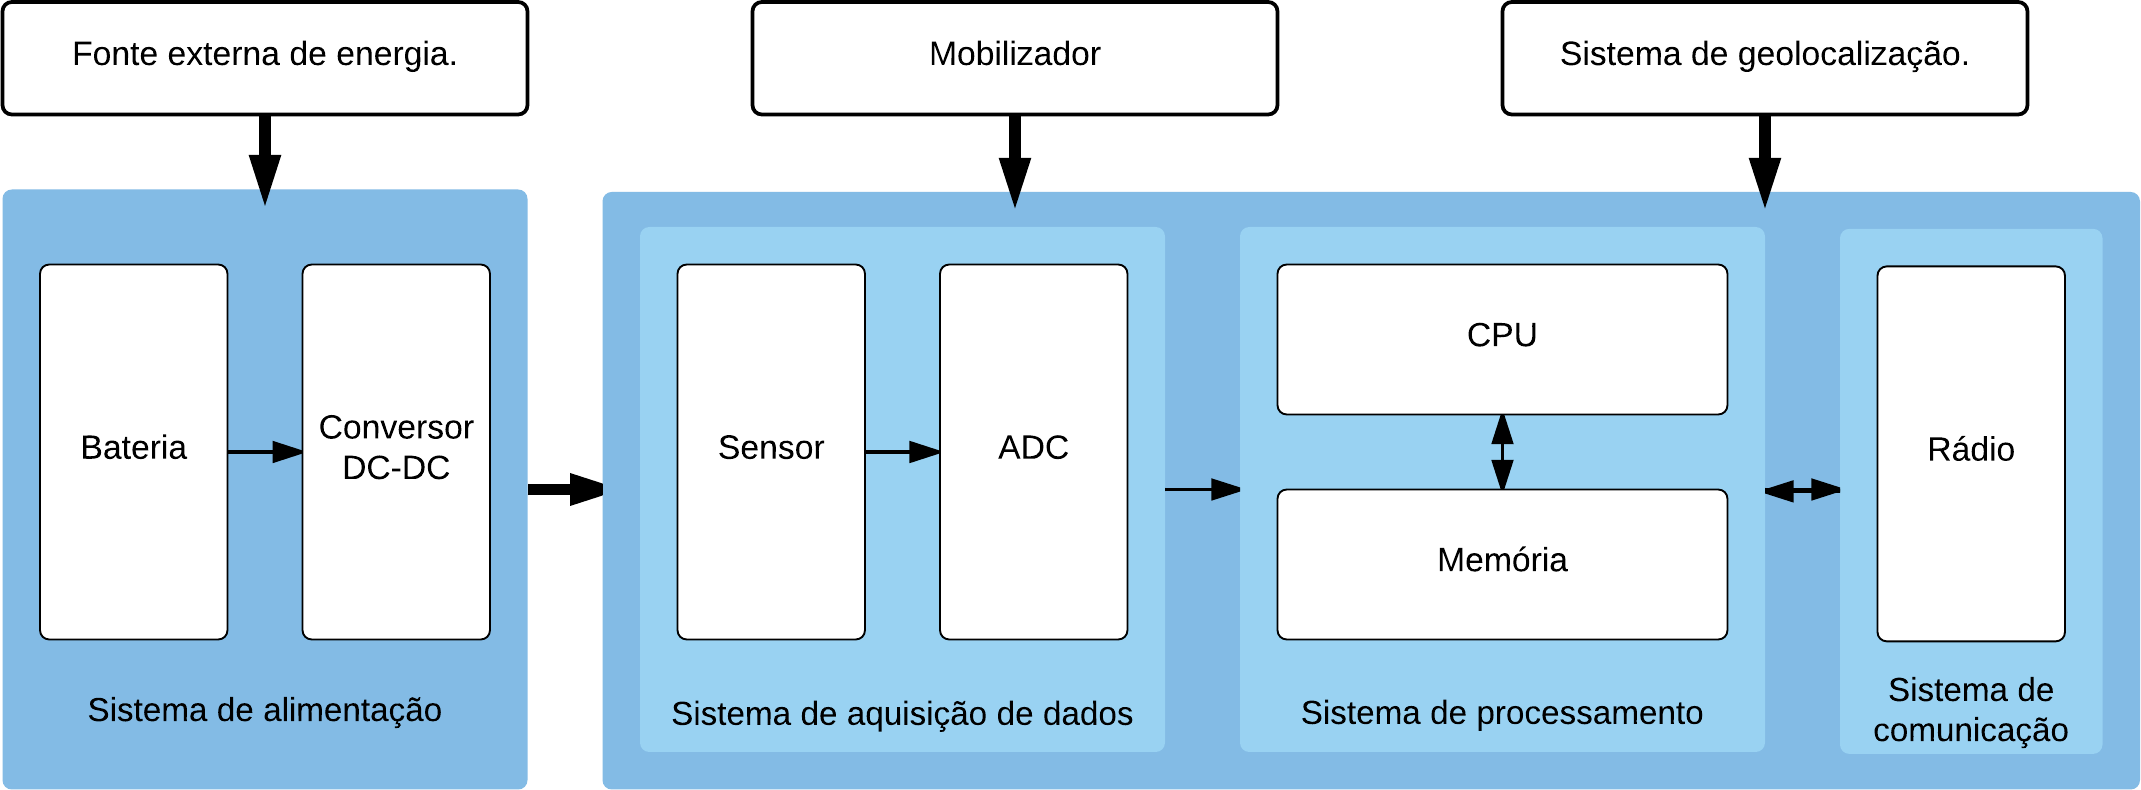
\includegraphics[width=\linewidth]{SensorNode_Generic}
	\end{center}
	\legend{Adaptado de \citeonline{Anastasi2009}}
\end{figure}

Cada nodo de sensor representado por esta arquitetura é composto essencialmente por quatro subsistemas \cite{Akyildiz2002, Rawat2014}.

\begin{itemize}
	\item \textit{Sistema de alimentação.} Responsável pelo fornecimento de energia aos demais componentes, deve regular a voltagem e realizar outras adequações que se façam necessárias nas linhas de alimentação do nodo. Pode ainda realizar a captura e o armazenamento da energia proveniente de fontes externas secundárias, quando disponíveis. É essencialmente composto por uma ou mais baterias primárias e um conversor DC-DC, capaz de manter, de forma eficiente, os níveis de voltagem adequados nas linhas de alimentação.
	\item \textit{Sistema de aquisição de dados.} É capaz de obter, quando solicitado, dados amostrais a partir dos fenômenos monitorados. Deve contar com um ou mais transdutores, responsáveis por converter as grandezas físicas monitoradas em sinais elétricos analógicos. E com circuitos de conversão analógico-digital (ADC's), cujo propósito é realizar a conversão dos sinais analógicos, provenientes dos transdutores, para sinais digitais compatíveis com as interfaces do sistema de processamento.
	\item \textit{Sistema de processamento.} É responsável por coordenar as tarefas delegadas ao nodo como, por exemplo, a obtenção de dados amostrais ou o roteamento de pacotes de dados encaminhados por outros nodos. Este sistema é composto essencialmente por um microcontrolador com memória integrada e pode, opcionalmente, contar com módulos de memória adicionais, a fim de permitir o armazenamento de maiores quantidades de dados. O que pode vir a ser necessário de acordo com a topologia da rede ou caso não haja disponibilidade de conexões com o exterior.
	\item \textit{Sistema de comunicação.} É o responsável por permitir que os dados trafeguem entre os nodos que compõem a rede. Sua implementação mais comum, e a que será considerada ao longo deste trabalho, se baseia na utilização de radiotransmissores de baixa potência. No entanto vale ressaltar que as possibilidades de implementação não se restringem somente a este método. Em casos específicos, e onde a transmissão via rádio não é vantajosa, factível ou financeiramente viável, outros métodos de comunicação, como infra-vermelho ou transmissores acústicos, podem ser utilizados.
\end{itemize}

Algumas aplicações podem ainda requerer sistemas adicionais, como, por exemplo: mecanismos de geolocalização (capazes de determinar a localização geográfica de determinado nodo); sistemas de mobilização (capazes de mover os nodos equipados entre diferentes posições, ou ainda, de reorientar antenas direcionais); sistemas de localização relativa (capazes de determinar a posição de um nodo em relação aos demais). A implementação destes sistemas pode tanto requerer hardware adicional ou permitir que sejam implementados puramente em software. No entanto, por se tratarem de componentes raramente utilizados, não serão considerados parte integrante deste modelo básico.

Existem ainda os \textit{gateways} e \textit{sinks}, cuja arquitetura básica se assemelha à presente nos demais nodos. No entanto \textit{gateways} devem contar com interfaces de comunicação secundárias, capazes de estabelecer conexão entre a rede de sensores e alguma rede externa, ou diretamente com a internet. Já os \textit{sinks}, devem ser capazes de armazenar maior quantidade de dados localmente. Ambos frequentemente possuem maior poder de processamento, a fim de permitir que lidem com a carga extra de trabalho sem criar gargalos. Geralmente as funções de \textit{sink} e \textit{gateway} são atribuídas aos mesmos nodos, facilitando a coleta ou transferência dos dados coletados.

Para melhor compreender os desafios com os quais as propostas realizadas nas seções \ref{phynode} e \ref{phymac} visam lidar, certos aspectos específicos da operação dos nodos devem ser esclarecidos. A seguir serão melhor discutidas algumas peculiaridades e métodos relacionados à conservação de energia, protocolos de roteamento e estimativa de qualidade dos links de rádio, nas redes de sensores sem fios. Serão também analisadas iniciativas realizadas no sentido de fornecer padrões de implementação e operação.

\section{Conservação de energia}
A distribuição do consumo energético dentre os diferentes subsistemas, bem como as rotinas empregadas para transmissão e aquisição de dados, estão parcialmente sujeitas aos requisitos específicos das aplicações. No entanto algumas observações gerais são aplicáveis à maioria dos sistemas.

\begin{itemize}
	\item O consumo apresentado pelos sistemas de comunicação é muito superior ao originado no sistema de processamento. Sendo a energia utilizada para transmitir um único bit via rádio equivalente à empregada no processamento de até mil instruções, num nodo típico \cite{Pottie2000}. Sendo assim, é mais vantajoso aplicar processamento local, a fim de reduzir o volume de dados a ser transmitido, do que transmitir grandes quantidades de dados brutos.
	\item O consumo energético apresentado pelos transmissores de rádio nos modos de recepção, transmissão e espera é da mesma ordem. Existem, no entanto, em grande parte dos transmissores mais recentes, modos de baixo consumo cuja utilização, apesar de geralmente resultar em certa latência adicional, deve ser priorizada sempre que os protocolos de rede permitirem. Uma vez que resultam em expressivas reduções do consumo de energia no estado de espera.
	\item O consumo do sistema de aquisição de dados é altamente dependente dos requisitos da aplicação, sendo em muitos casos significativo, e até mesmo superior ao consumo do sistema de comunicação. Nestes casos, torna-se interessante utilizar algoritmos destinados especificamente a minimizar o consumo referente à coleta de dados.
\end{itemize}

\begin{figure}[htb]
	\caption{\label{fig_energy_conservation}Técnicas para conservação de energia}
	\begin{center}
		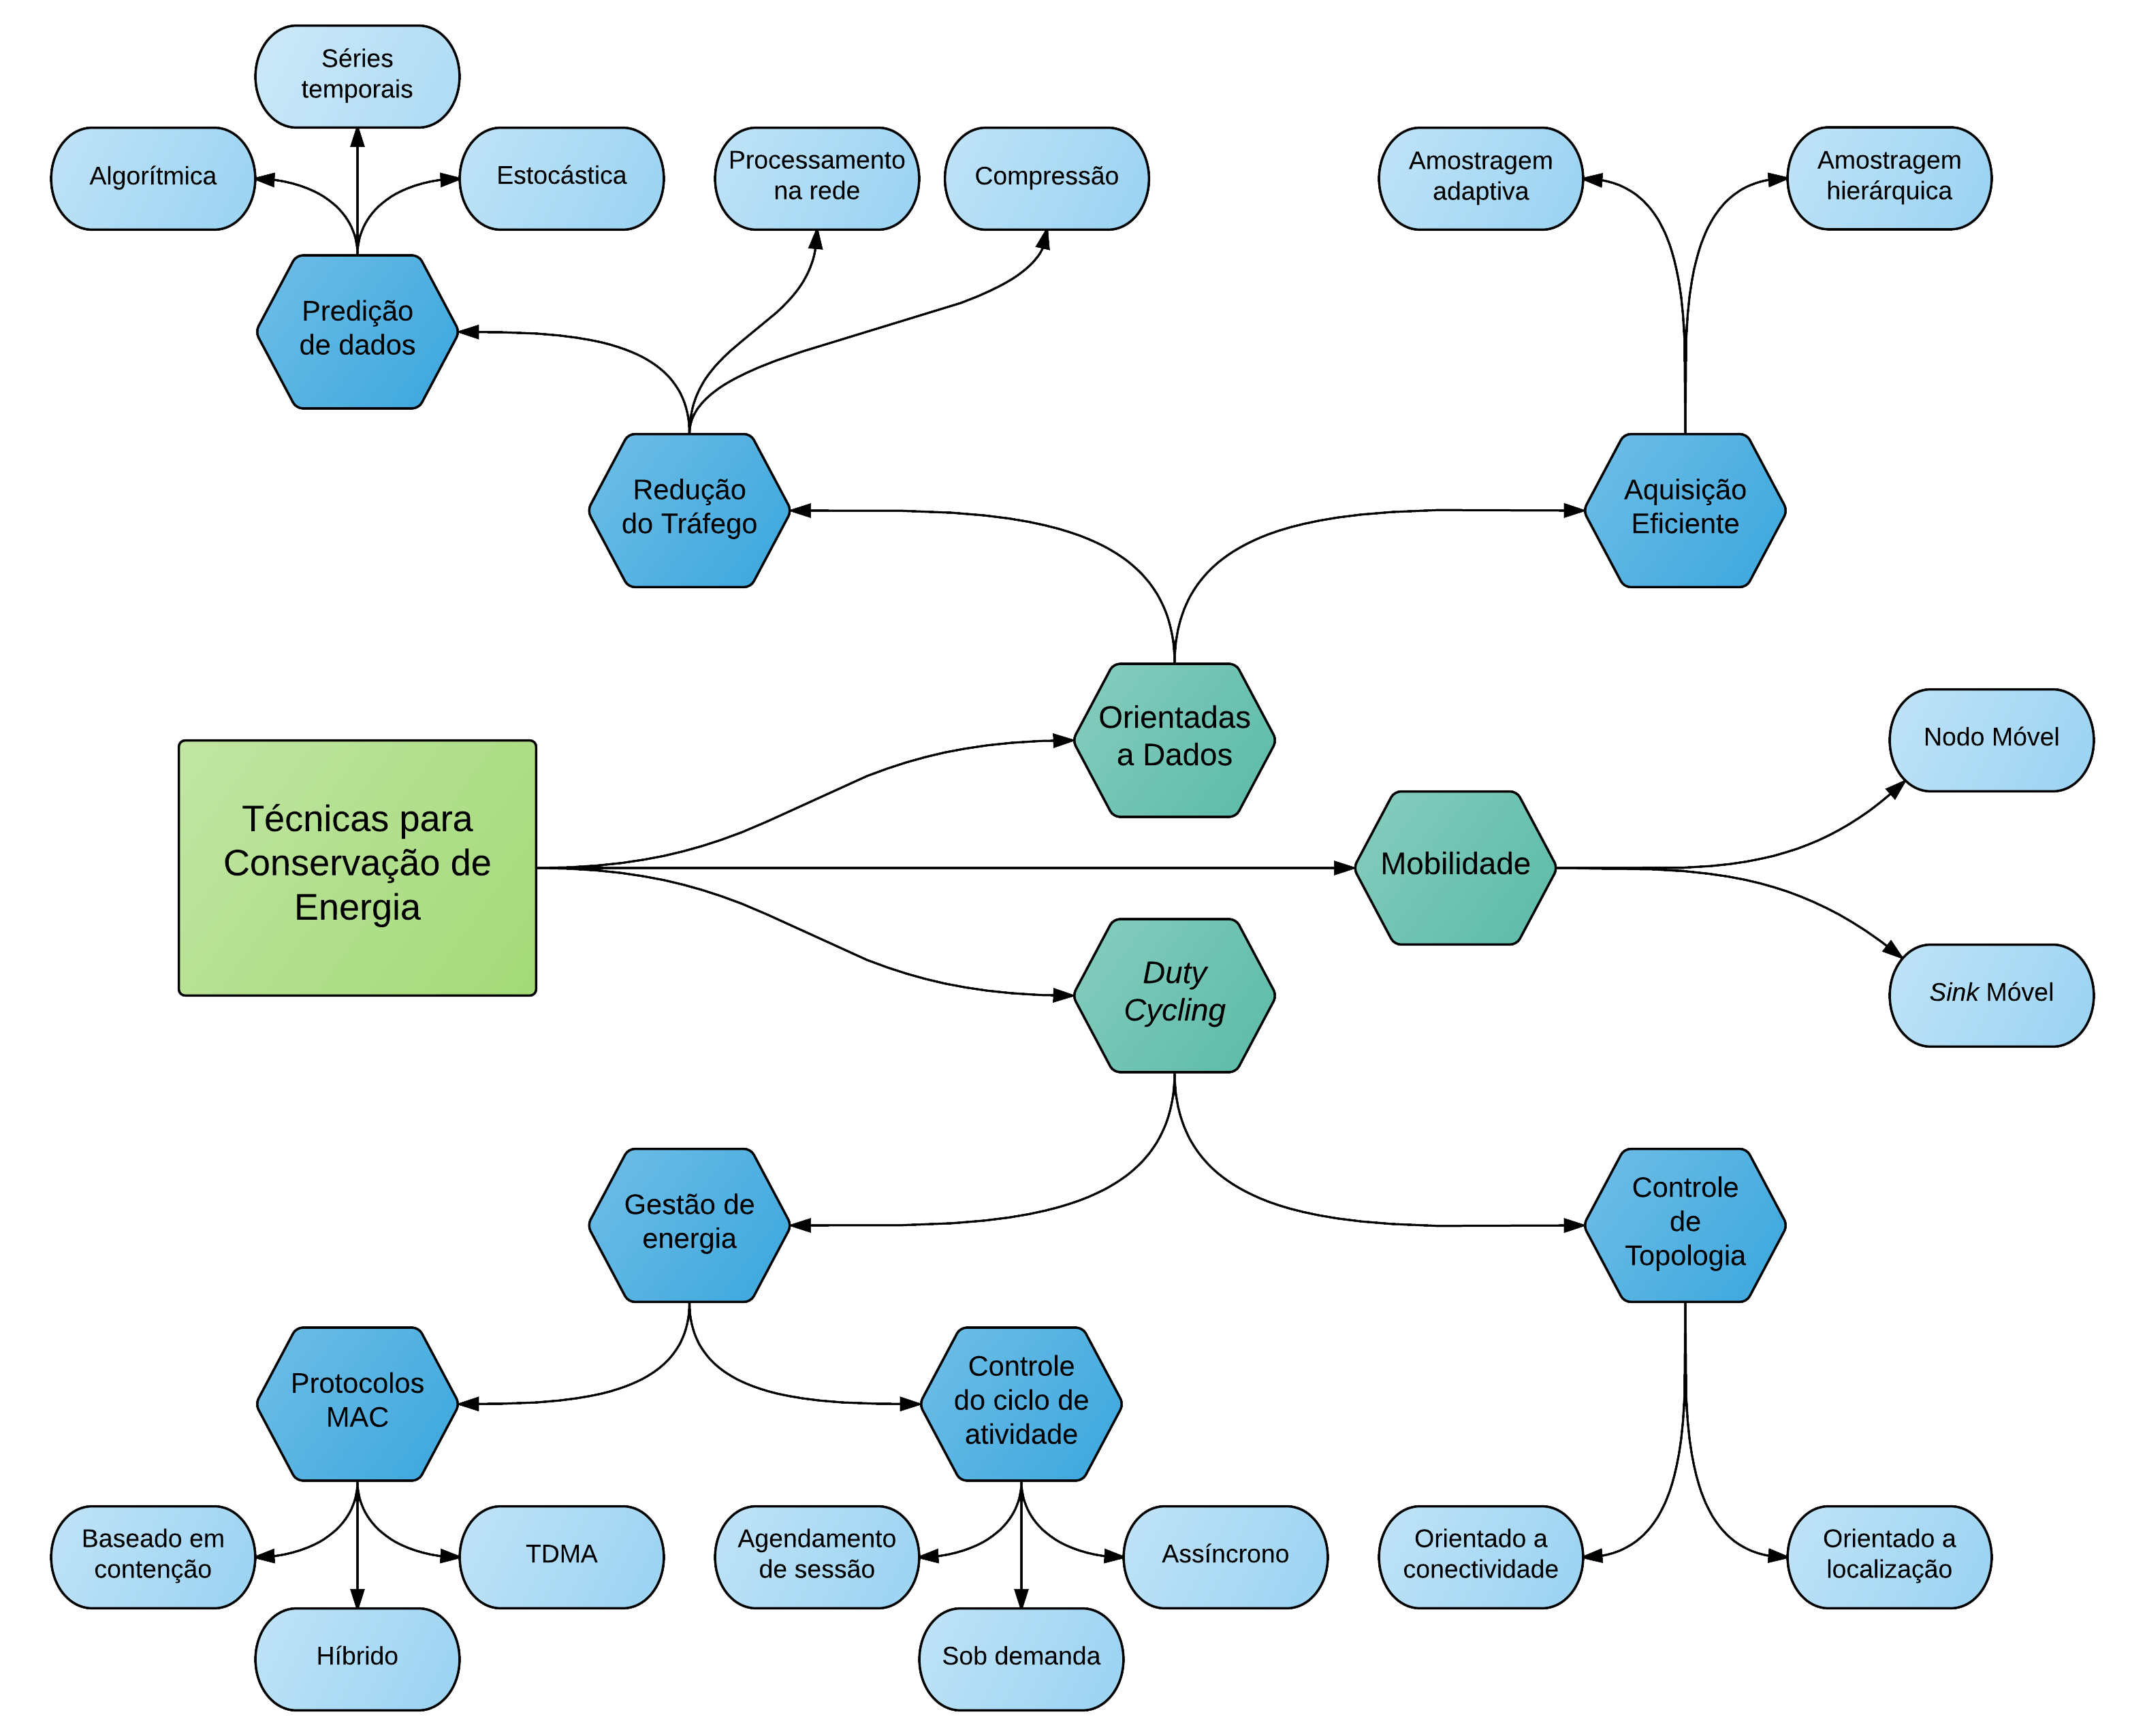
\includegraphics[width=\linewidth]{EnergyConservation}
	\end{center}
	\legend{Adaptado de \citeonline{Anastasi2009}}
\end{figure}

Baseando-se nestas premissas é possível explorar diversas abordagens para otimizar o consumo de energia nos nodos de sensor. A \autoref{fig_energy_conservation} apresenta uma classificação hierárquica destas técnicas, como proposta em \cite{Anastasi2009}. Embora mais de uma dezena de técnicas específicas sejam apresentadas, conceitualmente estas abordagens podem ser todas classificadas em três subcategorias principais: técnicas baseadas em \textit{duty-cycling}, técnicas orientadas a dados e técnicas orientadas a mobilidade.

\subsection{Técnicas baseadas em \textit{duty-cycling}}

Técnicas baseadas em \textit{duty-cycling} consistem em estabelecer estratégias para que determinados sistemas dos nodos possam, periodicamente, ser desativados ou colocados em estados de baixo consumo. Possibilitando desta maneira que haja uma redução na média de consumo energético do sistema em questão. O período de atividade, ou \textit{duty-cycle}, é um valor percentual que representa a fração de tempo durante a qual este subsistema deverá manter-se ativo dentro de um determinado período de tempo.

Embora também possam ser aplicadas aos demais sistemas, técnicas desta natureza são comumente utilizadas para o controle do sistema de comunicação, dado que neste caso podem proporcionar melhorias significativas devido ao alto consumo deste sistema. Contudo o aumento na latência dos links de comunicação, ocasionado pela indisponibilidade dos transceptores durante os períodos em que são colocados em modos de baixo consumo, faz com que esta abordagem não seja adequada em todas as situações. Convenientemente em alguns casos é possível variar o \textit{duty-cycle} dinamicamente, de acordo com a intensidade do tráfego, por exemplo, a fim de proporcionar um melhor comprometimento entre a redução do consumo de energia e a latência dos links de comunicação.

\subsection{Técnicas orientadas a dados}

Apesar de as técnicas baseadas em \textit{duty-cycling} possibilitarem alguma redução no consumo de energia ao impedir que certos sistemas do nodo permaneçam em modos de alto consumo durante períodos de inatividade, por definição elas não dispõem dos meios para análise dos dados coletados pelo sensores ou retransmitidos pelos nodos. Assim sendo, ignoram quaisquer redundâncias presentes nas informações que circulam pela rede, potencialmente permitindo que alguma energia seja desperdiçada durante a manipulação de dados essencialmente desnecessários. Já as técnicas orientadas a dados são especificamente destinadas a analisar estes dados, de forma a eliminar possíveis redundâncias e evitar ciclos de amostragem ou retransmissões desnecessárias. Estas técnicas operam na camada de aplicação, sendo geralmente utilizadas em conjunto com outros métodos, operando em camadas inferiores, a fim de reduzir ainda mais o consumo energético das redes de sensores.

Mais especificamente, a ausência de métodos destinados ao controle de redundâncias afeta a eficiência energética da rede permitindo que dois tipos distintos de evento ocorram:

\begin{itemize}
	\item \textit{Transmissão de dados redundantes.} Dados amostrais geralmente apresentam forte correlação espacial e temporal logo, para satisfazer os requisitos de determinadas aplicações, pode não ser necessário transmitir na íntegra todas as amostras coletadas. É possível ainda aplicar técnicas de agregação e compressão de dados a fim de reduzir o volume de tráfego sem omitir amostras já coletadas.
	\item \textit{Aquisição de dados redundantes.} Alguns sistemas de aquisição apresentam alto consumo de energia, nestes casos o ideal é evitar, sempre que possível, que sejam realizados ciclos de amostragem desnecessários. Para tal geralmente são empregados algoritmos especializados, responsáveis por verificar se dados equivalentes foram previamente coletados (localmente ou por nodos próximos) antes que se iniciem novas amostragens.
\end{itemize}

\subsection{Técnicas orientadas à mobilidade}

Existem ainda técnicas de conservação de energia baseadas na mobilidade de nodos. Durante sua operação de rotina, os nodos de uma rede de sensores sem fios conduzem os dados coletados em direção aos \textit{sinks}. A principal consequência deste paradigma é a sobrecarga dos meios de transmissão dos nodos localizados próximo aos \textit{sinks}, através dos quais deverão trafegar na íntegra todos os dados coletados pela rede \cite{Li2007}. A sobrecarga dos meios de transmissão nesta região provoca um consumo acelerado das reservas de energia dos nodos envolvidos: em geral os protocolos de comunicação se tornam menos eficientes em regiões sobrecarregadas, devido a maior probabilidade de ocorrerem colisões e, consequentemente um maior número de tentativas de retransmissão. A exaustão prematura das fontes de energia destes nodos, por sua vez, pode levar à subutilização de nodos mais distantes que, apesar de não terem suas reservas energéticas esgotadas, são inutilizados caso deixem de dispor de rotas de acesso aos \textit{sinks}.

Neste contexto, nodos ou \textit{sinks} móveis podem ser utilizados a fim de mitigar a sobrecarga de certas regiões, realizando a coleta dos dados enquanto se movimentam através da rede. Esta abordagem exige que os nodos estáticos fiquem à espera da passagem dos nodos móveis, quando terão a oportunidade de transmitir os dados diretamente a um \textit{sink} móvel, ou através de rotas mais eficientes. Este processo beneficia o balanceamento de cargas e possibilita uma utilização mais uniforme das reservas de energia de todos os nodos estáticos. Ao eliminar regiões potencialmente sobrecarregadas é possível ainda obter algum aumento na eficiência dos protocolos de comunicação, devido à redução dos níveis de contenção (tentativas frustradas de acesso aos meios de transmissão). Para que estas abordagens sejam efetivas, no entanto, deve-se planejar cuidadosamente os padrões de movimentação dos nodos móveis. Caso se torne muito complexo ou dispendioso projetar nodos móveis customizados, existe ainda a possibilidade de utilizar-se de entidades que já se movimentem pela área monitorada, como veículos ou animais.

\section{Estimativa de qualidade  dos links}

A propagação dos sinais de rádio, principalmente nos links de baixa potência como os utilizados nas redes de sensores sem fios, é significativamente afetada por diversos fatores externos que contribuem para sua degradação. O que faz com que estes links se comportem de forma errática, sendo que sua performance pode variar ao longo do tempo, e de acordo com a localização dos nodos. Falhas de transmissão, como o corrompimento ou perda dos pacotes de dados e as ações subsequentes, destinadas à correção destas falhas, chegam a ser responsáveis por 50\% a 80\% do consumo de energia proveniente dos sistemas de comunicação, variando de acordo com a intensidade do tráfego \cite{Srinivasan2006}. Além de prejudicar a execução de protocolos de mais alto nível, uma vez que a largura de banda disponível é efetivamente reduzida e inviabiliza-se transações que imponham restrições temporais rigorosas.

As perturbações responsáveis por degradar a qualidade dos links são causadas por fenômenos cujo comportamento e origens são bastante distintos. No entanto podem ser classificadas quanto à sua natureza em duas principais categorias: atenuação e interferência. Entende-se por atenuação a absorção ou reflexão parcial, em decorrência da interação dos sinais de rádio emitidos por um transmissor com o ambiente. O que resulta numa redução da intensidade do sinal captado pelo receptor. Já o termo interferência se refere ao acoplamento de sinais externos, e de frequência similar, às transmissões realizada entre um transmissor e um receptor. Este processo causa distorções no sinal original e resulta no corrompimento dos dados transmitidos sem que haja, necessariamente, qualquer redução na intensidade do sinal captado pelo receptor. De acordo com \cite{Baccour2012} são três os principais fatores que exercem influência sobre a qualidade dos links de rádio:
\begin{itemize}
	\item \textit{O ambiente.} Além de ser o principal componente para a atenuação dos sinais, também é responsável pela ocorrência do fenômeno conhecido como propagação multicaminho. Que ocorre quando, ao se propagar através de certo ambiente, componentes parciais de um mesmo sinal são refletidos e dispersam-se através de múltiplas rotas, cada um deles atingindo o receptor com diferentes intensidades e ligeira defasagem temporal \cite{Kusy2011}. O que resulta na distorção do sinal original e leva ao corrompimento dos dados. O ambiente também determina os níveis de ruído de fundo, contribuindo para determinação da relação entre sinal e ruído.
	\item \textit{O hardware.} Transmissores de rádio invariavelmente apresenta alguma variabilidade nos níveis de sinal, devido a seu próprio ruído interno e às faixas de tolerância aplicadas aos valores dos componentes utilizados para sua construção \cite{Goldsmith2005}. Com o desenvolvimento de hardware mais atualizado, este fator tende a exercer menor influência sobre a qualidade final dos links, porém não deve ser desconsiderado durante a concepção de métodos de estimativa de qualidade ou protocolos de comunicação. 
	\item \textit{Interferência.} É causada pela presença de múltiplos sinais sendo transmitidos concorrentemente, num mesmo ambiente, através de faixas de frequência similares. Podendo inclusive estes sinais originarem-se em diferentes nodos de uma mesma rede de sensores sem fios. Segundo \cite{Baccour2012} a área sobre a qual transmissões de um nodo podem causar interferência destrutiva supera a área na qual este nodo consegue manter links de comunicação confiáveis, logo podem-se estabelecer relações de interferência mesmo entre nodos que não sejam vizinhos diretos. Fontes de interferência podem ainda incluir outros equipamentos que compartilhem as mesmas faixas de frequência para comunicação sem fios e ruído eletromagnético gerado involuntariamente por certos equipamentos elétricos.
\end{itemize}

Nas redes de sensores sem fios, ao contrário do que acontece em outros ambientes, as aplicações finais não podem desacoplar completamente suas atividades dos processos de comunicação. Estas aplicações e os protocolos de rede por elas empregados devem, a fim de otimizar seus processos, levar em consideração a qualidade dos links disponíveis. Estimativas de qualidade acuradas podem auxiliar no processo de seleção de rotas mais eficientes, caso existam \cite{YanjunLi2005}. Ou ainda serem utilizadas para determinar os momentos mais apropriados para transmissão de dados, nos quais haverá maior probabilidade de sucesso \cite{Srinivasan2008}. Alternativamente, quando disponibilizadas a processos de mais alto nível, estas estimativas podem também ser utilizadas para adequar certas rotinas à qualidade momentânea dos links. Permitindo por exemplo alterações dinâmicas nas frequências de aquisição de dados, ou no comportamento de mecanismos de compressão ou agregação de dados, que podem se adequar à banda disponível.

\subsection{Etapas do processo de estimativa}

Entende-se por estimativa da qualidade de um link como a avaliação de uma métrica, definida matematicamente a partir de parâmetros relevantes, e aplicada sobre um conjunto de dados amostrais. O qual pode ser composto por uma quantidade predefinida de amostras, ou por uma quantidade variável de amostras coletadas durante um período predefinido de tempo. Geralmente refere-se a esta métrica como LQE (\textit{Link Quality Estimator}). Para que seja possível realizar a estimativa é necessário que sejam realizadas medições no link, por exemplo, através do registro dos números de sequência dos pacotes recebidos ou da aferição da intensidade do sinal durante a recepção dos pacotes de dados. É necessário ainda que se defina um método de monitoramento, responsável por garantir que haverá uma quantidade mínima de tráfego no link, a fim de permitir que as medições possam ser realizadas com frequência regular. O processo completo de estimativa de qualidade consiste, portanto, em três atividades distintas: monitoramento do link, medições no link e avaliação da métrica \cite{Baccour2012}. Estas atividades são ilustradas na \autoref{fig_lqe_steps}.

\begin{figure}[htb]
	\caption{\label{fig_lqe_steps}Processo de estimativa de qualidade do link.}
	\begin{center}
		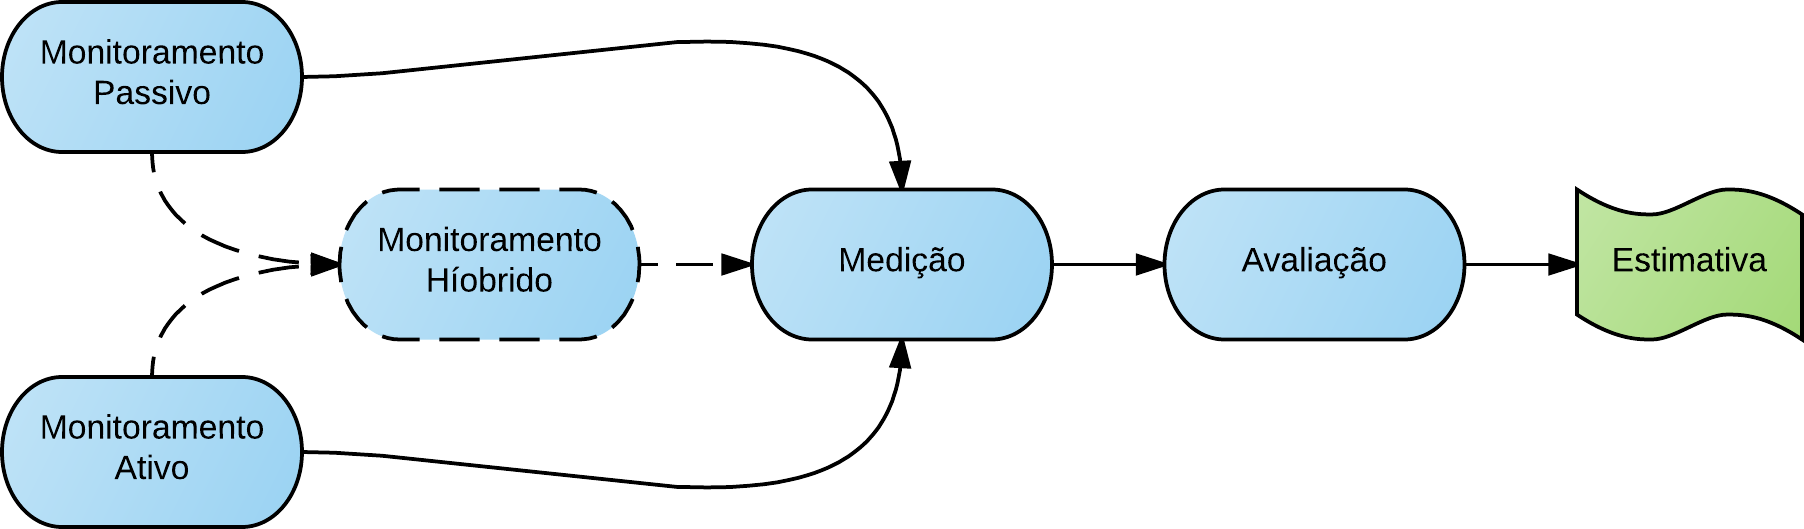
\includegraphics[width=\linewidth]{WSN_LQE_Steps}
	\end{center}
	\legend{Adaptado de \citeonline{Baccour2012}}
\end{figure}

A primeira atividade, monitoramento do link, pode ser realizada baseando-se em três diferentes abordagens: monitoramento ativo, passivo ou híbrido. As informações obtidas pelos mecanismos de monitoramento, além de permitirem a coleta de dados para estimativa de qualidade dos links, podem ser consumidas por outros algoritmos relacionados aos processos de roteamento ou controle de topologia.

O monitoramento ativo é realizado através da troca de pacotes de teste, denominados \textit{beacons}, entre os nodos e seus vizinhos. Estes pacotes podem ser transmitidos via \textit{broadcast} \cite{DeCouto2005} ou \textit{unicast} \cite{Kim2006}. Mecanismos baseados em \textit{broadcast} tem a vantagem de não requererem \textit{feedback}, por parte dos destinatários, quanto ao recebimento dos \textit{beacons}. O que permite implementações mais simples, se comparado aos mecanismos baseados em \textit{unicast}, e evita possíveis retransmissões automáticas por parte da camada de \textit{link}. Já as alternativas baseadas em \textit{unicast} proporcionam a obtenção de dados mais acurados, uma vez que utilizam pacotes semelhantes ao tráfego real \cite{Sang2010} e são capazes de identificar possíveis assimetrias nos links. Entretanto mecanismos baseados em \textit{unicast} tendem a consumir uma quantidade maior de recursos do sistema de comunicação.

O monitoramento passivo explora o tráfego usual da rede para computar as estatísticas de conectividade. Com isto reduz-se a utilização de banda e o consumo de energia associados à transmissão dos \textit{beacons}. Caso o tráfego envolvendo um único nodo não seja suficiente para manter suas estimativas atualizadas pode-se utilizar a técnica conhecida como \textit{sniffing}, que consiste em capturar todos os pacotes que trafegam nas proximidades, permitindo a obtenção de um volume maior de informações \cite{LaI2003,Woo2003}. É possível ainda capturar somente as confirmações de recebimento emitidas por nodos vizinhos, aproveitando-se de \textit{beacons} emitidos por outros nodos \cite{PengJiang2006,YanjunLi2005}. A utilização de técnicas de \textit{sniffing}, no entanto, exige que os módulos de rádio sejam mantidos em modo de escuta por períodos maiores, elevando o consumo energético do sistema de comunicação \cite{LaI2003}. Adicionalmente, em redes onde o volume de tráfego é reduzido ou desbalanceado, o monitoramento passivo pode criar uma deficiência de medições atualizadas, levando a estimativas de qualidade imprecisas \cite{Baccour2012}.

Existe ainda a possibilidade de utilizar métodos que combinem as técnicas de monitoramento ativo e passivo, permitindo melhores relações entre consumo de energia e obtenção de estimativas atualizadas \cite{Gnawali2009,Kim2006}. Geralmente estas técnicas, denominadas híbridas, consistem em utilizar o monitoramento passivo durante os períodos em que o volume de tráfego real permitir a obtenção de medições suficientemente atualizadas, alternando para mecanismos de monitoramento ativo quando o tráfego preexistente não for suficiente para manter as estimativas precisas para todos os nodos.

A segunda atividade relacionada ao processo de estimativa de qualidade consiste em realizar medições a partir dos dados obtidos na etapa anterior. As atividades realizadas nesta etapa envolvem computar parâmetros que não podem ser obtidos diretamente durante o monitoramento dos links, porém podem ser deduzidos a partir dos dados coletados. Parâmetros como, por exemplo, a relação sinal-ruído (\textit{Signal to Noise Ratio} ou SNR), taxas de recebimento ou perda de pacotes, podem ser computados nesta fase. É importante notar que os parâmetros monitorados pelos emissores e receptores, através das atividades de monitoramento, não são os mesmos. Contadores de retransmissão, por exemplo, estão disponíveis somente nos emissores. Já medições de intensidade do sinal recebido estão presentes somente nos receptores. Portanto técnicas de medição diferentes devem ser aplicadas a cada uma das extremidades do link.

A última etapa deste processo consiste em utilizar os dados provenientes da atividade de medição para avaliação de uma métrica (LQE), através da qual obtém-se a estimativa de qualidade do link. Os LQEs mais básicos podem ser subdivididos em duas categorias: baseados em software ou hardware. LQEs baseados puramente em hardware geram estimativas a partir de parâmetros associados à integridade do sinal, os mais comuns são: SNR, RSSI (\textit{Received Signal Strength Indicator}) e LQI (\textit{Link Quality Indicator}). Já os LQEs baseados puramente em software como, por exemplo, PRR (\textit{Packet Reception Ratio}) ou RNP (\textit{Required Number of Packets}), avaliam parâmetros relacionados à integridade dos pacotes recebidos \cite{Baccour2012}.

No entanto a confiabilidade dos estimadores citados acima é bastante limitada, uma vez que consideram somente uma pequena quantidade de parâmetros como base para o cálculo dos resultados. A fim de obter estimativas mais acuradas em geral são utilizados LQEs mais abrangentes, capazes de considerar simultaneamente parâmetros provenientes tanto do hardware quanto do software. \textit{Four-bit}, um LQE proposto em \citeonline{Fonseca2007}, por exemplo, considera parâmetros provenientes das camadas de rede, link e física. Já \textit{Triangle Metric}, propsoto em \citeonline{Boano2010}, considera parâmetros provenientes tanto da camada física quanto da camada de controle de acesso ao meio. Há ainda LQEs como \textit{MetricMap}, proposto em \citeonline{Wang2007}, que utilizam técnicas de aprendizado de máquina, lógica \textit{fuzzy} e outras técnicas avançadas de processamento para aprimorar seus resultados.

\subsection{Requisitos para estimativa de qualidade dos links}

Certos requisitos devem ser satisfeitos para que um estimador de qualidade possa operar de forma eficiente:

\begin{enumerate}
	\item \textit{Eficiência energética.} Uma vez que considera-se o consumo de energia como sendo uma grande preocupação nas redes de sensores sem fios, estimadores de qualidade dos links não devem sobrecarregar os sistemas de processamento e devem requerer o mínimo possível de comunicação adicional. Sistemas ativos com altas taxas de amostragem, portanto, devem ser evitados.
	\item \textit{Acurácia.} Entende-se por acurácia como sendo a habilidade de um LQE para caracterizar corretamente o comportamento do link. Sua acurácia determinará a eficiência com que um LQE será capaz de otimizar a utilização dos links pelos protocolos de rede. Na teoria da estimativa define-se que um processo estimado possa ser comparado a um processo conhecido e real, através de técnicas estatísticas, devendo apresentar comportamentos similares. No entanto, tal comparação não é possível para a estimativa de qualidade dos links pois: (i) não há nenhuma métrica amplamente adotada como medida absoluta da qualidade de um link e (ii) a qualidade do link pode ser representada por valores de natureza arbitrária: alguns estimadores baseiam-se no cálculo da taxa de recepção de pacotes, outros na contagem do número de retransmissões necessárias, entre outros. 

	Contudo a acurácia de um LQE ainda pode ser avaliada indiretamente, isto é, utilizando-se métricas subordinadas aos efeitos da estimativa sobre a eficiência dos protocolos de rede \cite{Baccour2012}. Por exemplo, em \citeonline{Fonseca2007} são avaliados os efeitos da utilização do estimador \textit{Four-bit} sobre a performance do protocolo de coleta de dados CTP (\textit{Collection Tree Protocol}). Conclui-se que a utilização deste estimador promove melhorias na taxa de entrega de pacotes, comprovando que o estimador favorece a seleção consistente de links de melhor qualidade, logo possui boa acurácia. Uma outra abordagem é utilizada em \citeonline{Baccour2011}, onde a distribuição temporal das estimativas fornecidas por alguns estimadores é estatisticamente analisada a fim de determinar sua confiabilidade.
	\item \textit{Reatividade.} Considera-se como reatividade, a capacidade de um estimador para detectar e reagir rapidamente a mudanças perenes na rede \cite{KimM.2001}. Um LQE reativo permite que os protocolos de roteamento e o controle de topologia se adaptem rapidamente a alterações na conectividade dos nodos. O nível de reatividade de um LQE depende de dois fatores: (i) o conjunto de dados utilizados para estimativas e (ii) o método de monitoramento escolhido. Conjuntos de dados pequenos e métodos de monitoramento ativos, utilizando altas taxas de amostragem levam a LQEs reativos. No entanto é importante notar que alguns LQEs são naturalmente mais reativos que outros. LQEs avaliados no emissor demonstraram-se geralmente mais reativos que LQEs avaliados no receptor \cite{Baccour2011}.
	\item \textit{Estabilidade.} Refere-se a estabilidade como sendo a capacidade de um LQE tolerar transientes na qualidade dos links. É importante que estes transientes sejam filtrados a fim de evitar que protocolos de roteamento e controle de topologia executem, desnecessariamente, rotinas custosas destinadas a reorganizar a rede após alterações perenes na rede como, por exemplo, a reinicialização das  tabelas de roteamento. Estimadores estáveis podem ser obtidos através do monitoramento do link a longo prazo \cite{Lin2009}. A estabilidade pode ser aferida através do coeficiente de variação das estimativas de qualidade, computado através da razão entre o desvio padrão das estimativas e sua média \cite{Woo2003}. Ou ainda avaliando-se o impacto do LQE sobre as rotinas de roteamento. Tipicamente LQEs estáveis resultam em topologias estáveis, nas quais observam-se poucas reorganizações de rotas \cite{Baccour2009}.
\end{enumerate}

Para que um estimador opere de forma eficiente, deve adotar a relação apropriada entre estabilidade e reatividade, permitindo que o roteamento adote a utilização dos links de comunicação que apresentem melhor qualidade a curto e longo prazo. Geralmente estimadores de melhor desempenho combinam múltiplas métricas para obter esta relação \cite{Sang2010}, ou utilizam para tal uma modelagem matemática precisa do comportamento da rede \cite{Woo2003}.

\subsection{Mecanismos básicos para LQE}

A seguir serão apresentados os mecanismos básicos, utilizados para avaliação de diferentes características dos \textit{links} de rádio, através dos quais compõem-se sistemas de estimativa mais complexos. Porém, antes de entrar em detalhes a respeito destes mecanismos, é importante compreender quais são os fenômenos que eles buscam avaliar e como interferem na qualidade das comunicações entre nodos. Em \cite{Kusy2011} encontram-se destacados os modos de falha mais comuns nos links de baixa potência utilizados em RSSFs.

\begin{itemize}
	\item Falha por parte do receptor, ao detectar o preâmbulo de uma transmissão iniciada por outro nodo. Geralmente devido a uma instabilidade temporária no link, o destinatário pode não captar o preâmbulo, elemento responsável por sinalizar o início da transmissão de um pacote. Neste caso o pacote é completamente ignorado por seu destinatário e será, possivelmente, retransmitido.
	\item Falha, por parte do receptor, ao capturar corretamente os dados de um pacote durante seu recebimento. Geralmente ocorre devido à instabilidade no link durante a transmissão. Neste caso o pacote será recebido, porém irá falhar na verificação de integridade, e será posteriormente descartado. A confirmação de recebimento não será enviada, forçando o emissor a retransmitir o pacote.
	\item Falha, por parte do transmissor, ao captar a confirmação de recebimento de um pacote previamente enviado. Neste caso o receptor recebe e processa o pacote corretamente, no entanto alguma instabilidade afeta o link no momento em que a confirmação de recebimento está sendo transmitida. Na ausência de uma confirmação, o transmissor conclui erroneamente que o pacote não foi recebido corretamente. Geralmente são realizadas novas tentativas de transmissão.
\end{itemize}

\begin{figure}[htb]
	\caption{\label{fig_lqe_methods}Métodos para estimativa de qualidade dos links.}
	\begin{center}
		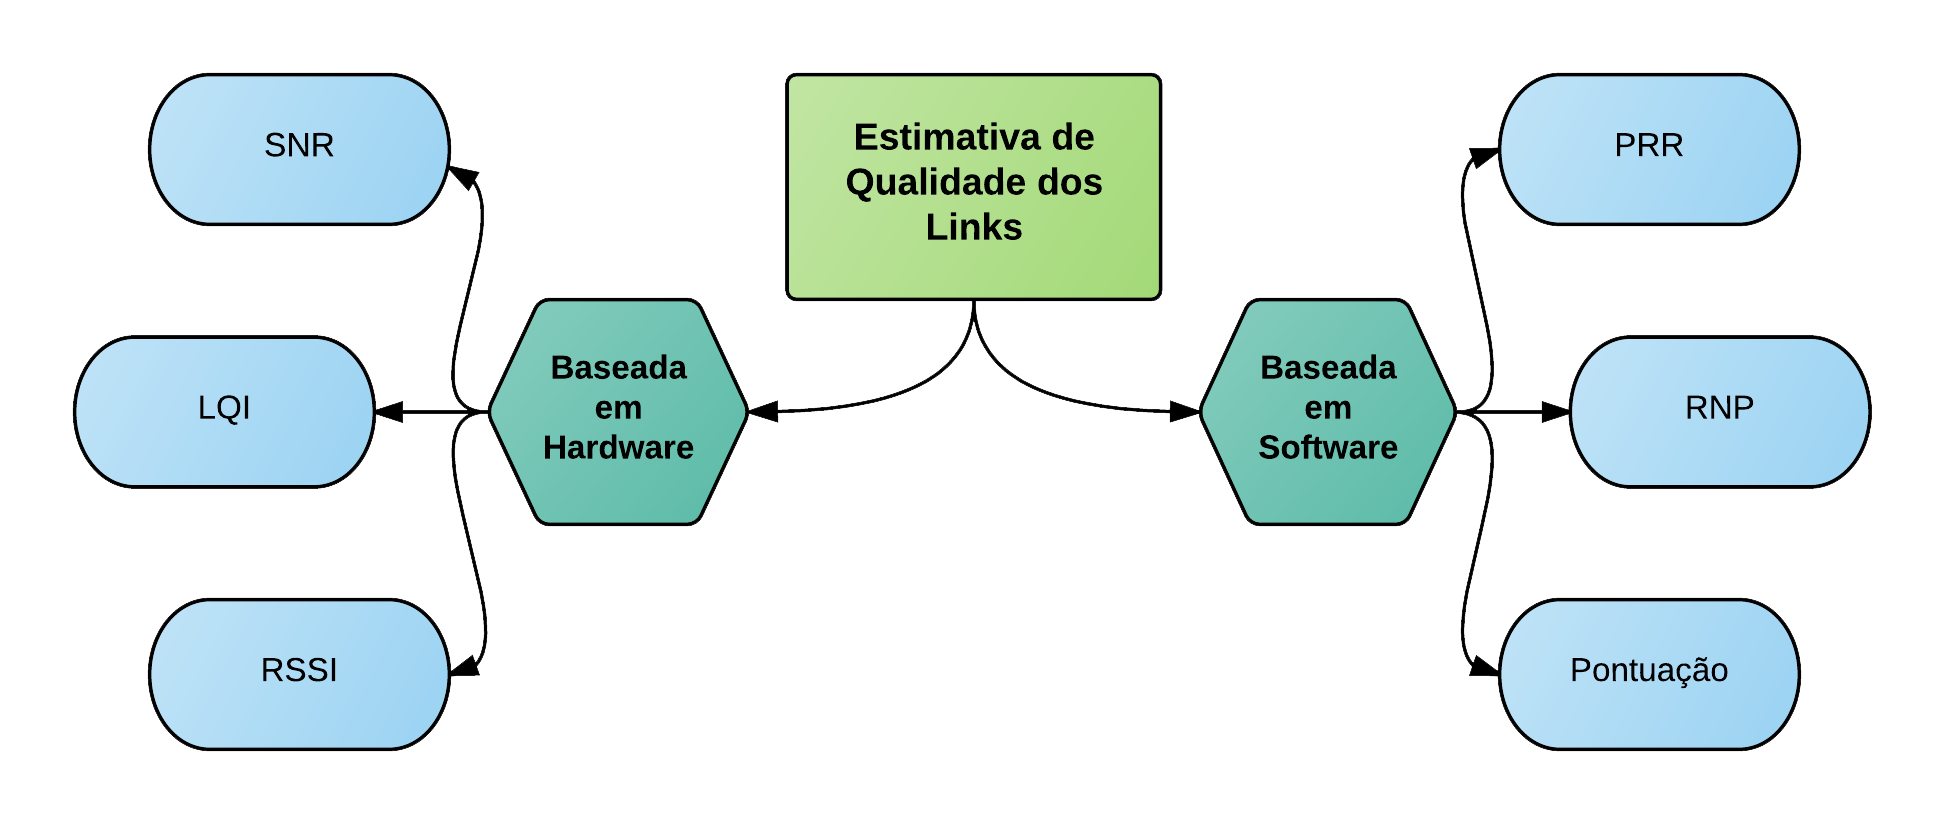
\includegraphics[width=\linewidth]{WSN_LQE_Methods}
	\end{center}
	\legend{Adaptado de \citeonline{Baccour2012}}
\end{figure}

Embora somente detectar e quantificar a presença de componentes de interferência, atenuação ou distorções causadas pela propagação multi-caminho sobre os sinais subjacentes não seja suficiente para estimar a qualidade de um link com a competência necessária para evitar estes modos de falha, estas informações são a base para avaliação de métricas mais completas. Os mecanismos básicos utilizados para obtê-las fim podem ser divididos em duas categorias básicas: baseados em \textit{hardware} e baseados em \textit{software}. Encontra-se ilustrada na \autoref{fig_lqe_methods} uma classificação para estes mecanismos. Em geral os mecanismos baseados em hardware são capazes de prover informações acuradas sobre determinadas propriedades físicas dos sinais recebidos, como intensidade do sinal (RSSI) ou relação sinal-ruído (SNR). No entanto não são adequados para avaliar o impacto destes componentes sobre a eficiência do link. Já os mecanismos baseados em software podem prover índices de mais alto nível, como contadores de retransmissão (RNP) ou taxa de recepção de pacotes (PRR). Contudo não são capazes de apontar os fatores de baixo nível responsáveis pelos resultados obtidos.

\subsubsection{Mecanismos baseados em hardware}

Os mecanismos de estimativa baseados em hardware provêm informações a respeito da qualidade dos sinais enquanto processados pelas camadas inferiores da pilha de protocolos. A implementação de tais mecanismos depende de hardware especializado, geralmente integrado ao \textit{frontend} analógico dos \textit{chips} de rádio. São três os principais mecanismos desta categoria: RSSI, SNR e LQI.

\begin{itemize}
	\item \textit{Radio Signal Strength Indicator (RSSI).} O RSSI provê uma medida instantânea da intensidade com que um sinal é recebido pelo módulo de rádio. Quando não há nenhuma transmissão em curso representa uma estimativa da intensidade do ruído de fundo \cite{Baccour2012}. A utilização do RSSI é atrativa por consistir numa forma simples e acessível de avaliar a qualidade do link entre dois nodos. No entanto, apesar de existir alta correlação entre baixa intensidade de sinal e falhas de transmissão, a afirmativa complementar pode não ser verdadeira. Mesmo links que possuam RSSI consistentemente elevados podem apresentar altas taxas de falha e perdas de pacotes \cite{Srinivasan2006}.
	\item \textit{Signal to Noise Ratio (SNR).} Esta métrica representa a intensidade do sinal recebido em relação ao nível de ruído de fundo. Isto a torna uma métrica mais acurada que o RSSI que, por sua vez, indica a intensidade do sinal recebido somada ao ruído de fundo. SNR é, portanto, mais capaz de estimar quais as chances de o sinal recebido ser decodificado corretamente, não importando sua intensidade \cite{Srinivasan2010}. No entanto o SNR só pode ser calculado a partir de pacotes detectados com sucesso, o que faz com que não seja confiável quando aplicado aos nodos de regiões transicionais \cite{LaI2003}. Nestas regiões os valores obtidos para o SNR podem ser tendenciosos, superestimando a qualidade do link, uma vez que não contabilizam os pacotes perdidos.
	\item \textit{Link Quality Indicator (LQI).} É uma métrica proposta no padrão IEEE 802.15.4 \cite{IEEE2003}, porém sua implementação pode variar de acordo com o fabricante e o \textit{chipset} escolhidos. O LQI pode indicar se um link apresenta excelente qualidade ou não. No entanto não é um bom indicador para links intermediários, apresentando alta variância nesta situações \cite{Baccour2012}. Aconselha-se utilizar a média dos resultados obtidos durante algum período para melhorar a qualidade das estimativas obtidas \cite{Srinivasan2006}. É possível ainda basear-se no LQI para estimar a qualidade do link indiretamente, utilizando sua variância como métrica final \cite{Boano2009}. Links de baixa qualidade apresentarão alta variância e links de boa qualidade apresentarão baixa variância. Esta técnica permite uma resposta mais rápida que o cálculo da média, pois permite que um resultado final seja obtido sem a necessidade de avaliar uma quantidade tão grande de pacotes. Adicionalmente os valores obtidos a partir deste mecanismo são de natureza arbitrária, podendo variar de acordo com a implementação utilizada por cada fabricante.
\end{itemize}
	
	Todos estes mecanismos, no entanto, compartilham algumas limitações. Primeiramente, só podem ser computados a partir de pacotes recebidos com sucesso; logo, tendem a superestimar a qualidade dos links que apresentem muitas perdas de pacotes, uma vez que as estatísticas referentes a estes pacotes são ignoradas. E adicionalmente, apesar de consistirem em métricas rápidas e de baixo custo para classificar links como bons ou ruins, não são capazes de fornecer estimativas mais refinadas \cite{Baccour2012}, geralmente não sendo suficientes para prover informações relevantes a respeito dos links situados nas regiões transitórias.
	
\subsubsection{Mecanismos baseados em software}

Os mecanismos baseados em software provêm informações a respeito do link a partir das camadas superiores da pilha de protocolos. São mais adequados que os mecanismos baseados em hardware para computar estatísticas globais, porém menos capazes de avaliar as condições instantâneas dos meios de transmissão. São três as principais abordagens para desenvolvimento dos mecanismos pertencentes a esta categoria: PRR, RNP, pontuação.

\begin{itemize}
	\item \textit{Packet Reception Ratio (PRR).} Representa a razão entre o número de pacotes recebidos com sucesso e o número total de pacotes transmitidos, podendo ser computada a partir dos número de sequência encontrados nos pacotes recebidos. Em alguns casos também é utilizada a métrica análoga e complementar PER (\textit{Packet Error Rate}), obtida a partir de: $PER = 1 - PRR$ \cite{Baccour2012}.
	\item \textit{Required Number of Packets (RNP).} Esta métrica é obtida através da contagem do número necessário de retransmissões realizadas para que cada pacote enviado seja entregue com sucesso ao destinatário. RNP assume retransmissões automáticas, por parte dos protocolos de roteamento, caso pacotes sejam perdidos \cite{Cerpa2005}. Uma abordagem semelhante é utilizada na métrica \textit{Acknowledge Reception Radio (ARR)}, que considera a relação entre o número total de pacotes transmitidos e o número de confirmações de recebimento coletadas \cite{Baccour2012}.
	\item \textit{Métricas baseadas em pontuação.} Existem ainda métricas que apresentam seus resultados através de uma escala de valores definidos arbitrariamente, expressas por valores adimensionais, sem que estejam necessariamente relacionados com algum fenômeno físico \cite{Baccour2012}.
\end{itemize}

\section{Iniciativas de padronização}

Como citado anteriormente, a grande diversidade de aplicações às quais se destinam as redes de sensores sem fios gera a demanda por tecnologias de comunicação bastante diversificadas. No entanto a propagação tardia desta tecnologia à segmentos de mercado que permitissem sua utilização em larga escala favoreceu a disseminação de uma grande quantidade de protocolos de escopo pouco abrangente, destinados a aplicações específicas e, consequentemente, pouco desenvolvidos. Desenvolveu-se de forma semelhante o hardware utilizado para implementação destes sistemas, o qual era até recentemente baseado em componentes de uso geral ou em componentes emprestados de outras aplicações. Isto se devia à pouca demanda existente para componentes especificamente destinados aos requisitos das redes de sensores sem fios, que não justificava o esforço de grandes fabricantes para disponibilizar ao mercado soluções específicas, e também ao fato de que componentes desta natureza não podem ser projetados ou produzidos em pequena escala com o objetivo de, por exemplo, integrarem somente uma solução experimental ou de pequena escala.

O cenário descrito acima trás certas consequências negativas para o ecossistema de desenvolvimento das redes de sensores sem fios. Mais especificamente: a proliferação de uma grande quantidade de protocolos pouco difundidos impõe uma barreira para a capacidade de interoperabilidade destes sistemas. Adicionalmente a utilização destes protocolos em aplicações isoladas ou de pequena escala faz com que não existam esforços significativamente abrangentes direcionados para seu aprimoramento. O que também desencoraja a disseminação de soluções de hardware especificamente destinadas à utilização nas redes de sensores sem fios e outros sistemas interconectados de baixa potência.

\begin{table}[hbt]
	\centering
	\caption{Camadas do modelo OSI}
	\label{tab_osi}
	\begin{tabular}{p{0.7cm}|p{3.0cm}|p{10.8cm}|}
		\cline{2-3}
		& \multicolumn{1}{c}{\cellcolor[HTML]{C0C0C0}\textbf{Camada}} & \multicolumn{1}{c}{\cellcolor[HTML]{C0C0C0}\textbf{Função}} \\[3ex] \hline
		\multicolumn{1}{|l|}{} & 7. Aplicação & Tarefas de alto nível, relacionadas aos propósitos específicos do sistema em questão. \\ \cline{2-3} 
		\multicolumn{1}{|l|}{} & 6. Apresentação & Tradução e encapsulamento dos dados que trafegam entre a camada 7, de aplicação, e as demais: codificação, compressão, criptografia. \\ \cline{2-3} 
		\multicolumn{1}{|l|}{} & 5. Sessão & Gerenciamento de fluxos de dados, sequenciamento dos segmentos transmitidos entre dois nodos da rede. \\ \cline{2-3} 
		\multicolumn{1}{|l|}{\multirow{-4}{*}{\rotatebox[origin=c]{90}{Aplicação}}} & 4. Transporte & Transmissão confiável de segmentos de dados entre dois pontos na rede: segmentação, multiplexação \\ \hline
		\multicolumn{1}{|l|}{} & \textbf{3. Rede} & Estruturação e gerenciamento das redes: endereçamento, roteamento e controle de tráfego. \\ \cline{2-3} 
		\multicolumn{1}{|l|}{} & \textbf{2. Enlace} & Transmissão confiável de pacotes entre dois nodos conectados através de um meio físico \\ \cline{2-3} 
		\multicolumn{1}{|c|}{\multirow{-3}{*}{\rotatebox[origin=c]{90}{Transporte}}} & \textbf{1. Física} & Transmissão e recepção de fluxos brutos através de um meio físico. \\ \hline
	\end{tabular}
	\legend{Fonte: elaboração prórpia.}
\end{table}

No entanto a demanda por iniciativas capazes de lidar com estes dilemas tem aumentado. O padrão IEEE 802.15.4 \cite{IEEE2003} foi especificamente concebido para utilização em sistemas de comunicação de baixa potência, baixo custo e que operem com baixas taxas de transferência, aos quais se refere como LR-WPANs (\textit{Low Rate Personal Area Networks}). Este padrão destina-se à aplicações que requeiram links de comunicação de curto alcance e alta eficiência energética, nele são especificadas implementações para as duas camadas inferiores da pilha de protocolos: a camada física (PHY) e a camada de enlace, ou controle de acesso ao meio (MAC), conforme definidas pelo modelo OSI (apresentado na \autoref{tab_osi}). A arquitetura das camadas superiores é deferida aos diversos protocolos que implementam o IEEE 802.15.4, como 6LoWPAN \cite{Montenegro2007}, ZigBee \cite{ZigBee2005}, WirelessHART \cite{Kim2008}.

O padrão IEEE 802.15.4 define dois tipos de nodos: dispositivos com funcionalidade completa (\textit{full-functioning device}, ou FFD) e dispositivos com funcionalidade reduzida (\textit{reduced-function device}, ou RFD). RFDs são dispositivos dotados de menor capacidade de processamento e memória, localizados nas extremidades das redes e cuja funcionalidade se resume a estabelecer comunicação com algum FFD. Já os FFDs são dispositivos com maior capacidade embarcada de processamento e capazes de implementar completamente o padrão, são responsáveis por coordenar as atividades de comunicação e roteamento. Também é definido no IEEE 802.15.4 o suporte a duas topologias de rede: estrela e \textit{peer-to-peer}. \cite{Rawat2014}. Ao utilizar a topologia estrela todos os nodos devem se comunicar com um dispositivo controlador central, do tipo FFD. Já através da topologia \textit{peer-to-peer} é possível estabelecer links de comunicação entre dois nodos quaisquer, o que permite que se produzam rede mais complexas, como por exemplo redes \textit{mesh}, onde diversos nodos dispostos de forma potencialmente irregular colaboram para estabelecer rotas de comunicação entre si, mesmo que não sejam capazes de se comunicar diretamente.

A versão original do padrão, IEEE 802.15.4-2003 \cite{IEEE2003}, propõe somente duas definições para a camada PHY, permitindo a operação nas faixas de 868 MHz e 915 MHz (através da modulação BPSK, com taxa máxima de transferência de 40 kbps), e na faixa de 2.4 GHz (através da modulação O-QPSK, com taxa máxima de transferência de 250kbps). No entanto, devido à sua crescente popularidade, ao longo do tempo diversas revisões e emendas foram adicionadas ao padrão, tendo como objetivo expandir as funcionalidades originalmente previstas pela camada MAC e, com maior frequência, agregar novas definições de camadas PHY.

A primeira revisão aprovada do padrão, publicada como IEEE 802.15.4-2006 \cite{IEEE2006}, ocorreu três anos após a aprovação da versão original. Esta revisão teve como objetivo a incorporação de suporte à duas novas definições para a camada PHY, a fim de permitir a utilização de taxas de transferência mais elevadas nas bandas de frequência de 868 MHz e 915 MHz. Tal aperfeiçoamento foi possível através da utilização das modulações O-QPSK e ASK que permitem, neste caso, a operação à taxas de 100 kbps e 250 kbps respectivamente. Ainda nesta revisão foram adicionadas definições para mecanismos de segurança e outros aprimoramentos na camada MAC, como o suporte para uma base de tempo compartilhada, agendamento do envio de \textit{beacons} e a sincronização de mensagens de \textit{broadcast}.

Apenas um ano após a aprovação desta revisão foi proposta sua primeira emenda, dando origem ao IEEE 802.15.4a \cite{IEEE2007}. Através desta emenda foram incorporadas mais duas especificações PHY opcionais: o \textit{Chirp Spread Spectrum} (CSS), capaz de elevar a taxa de transferência na faixa de 2450 MHz para 1000 kbps, e a Ultra-wide Band (UWB) destinada à operação nas faixs de 3 GHz, 5 GHz e 6 GHz a 10 GHz e capaz de fornecer taxas de transferência de até 27.4 Mbps.

Em se tratando de padronização dos meios de difusão via radiofrequência, o maior empecilho encontrado está relacionado às divergências presentes nas regulamentações locais existentes em cada país. A alocação de bandas de frequência pode variar de acordo com as leis de cada país, exigindo certa flexibilidade dos padrões que visem obter permissão para operar globalmente. No caso do IEEE 802.15.4, as definições de camada PHY são destinadas à operação nas bandas ISM (\textit{Industrial, Scientific an Medical}), bandas de frequência internacionalmente reservadas para fins industriais, científicos e médicos, não necessariamente relacionados à transmissão de dados e que, por este motivo, apresentam menor variabilidade quanto as bandas de frequência alocadas nas diferentes regiões do planeta. Adicionalmente, devido à finalidade para qual são destinadas, as regulamentações que incidem sobre as bandas ISM tendem a ser mais permissivas quanto à irradiação não licenciada.

O sinal de transmissão associado ao PHY \textit{Ultra-wide Band} (UWB) possui ocupação espectral instantânea superior a 500 MHz e largura fracionária de banda superior a 20\%, o que permite alta eficiência espectral e altas taxas de transferência com baixo consumo energético, além de proporcionar alta tolerância aos efeitos da propagação multi-caminho \cite{Porcino2003}. Estas características, no entanto, fazem com que UWB requeira maior largura de banda do que a disponibilizada nas faixas de frequência ISM, caracterizando-a como a única definição de camada PHY incorporada ao IEEE 802.15.4 a não ser destinada às bandas ISM. Adicionalmente, as técnicas de transmissão utilizadas por UWB baseiam-se em pulsos de rádio extremamente curtos, emitidos através de sequências periódicas, o que torna a tecnologia inadequada para utilização em ambientes perigosos, devido à emissão de pulsos de alta energia. UBW também não é adequada para transmissões de longa distância \cite{Rawat2014}.

Ainda com o intuito de possibilitar maior abrangência geográfica ao padrão, apenas dois anos após a aprovação da emenda IEEE 802.15.4a, foram introduzidas as emendas IEEE 802.15.4c \cite{IEEE802_15_4c} e IEEE 802.15.4d \cite{IEEE802_15_4d}, destinadas a introduzir novas definições para a camada PHY, compatíveis com a operação nas bandas de frequência ISM disponíveis na China e no Japão. IEEE 802.15.4c introduz definições para operação nas bandas de frequência 314-316 MHz, 430-434 MHz e 779-787 MHz, assim como adequações na camada MAC a fim de compatibilizar o padrão com as regulamentação vigente à época, na China. Já o IEEE 802.15.4d define o suporte à operação na banda de 950 MHz assim como adequações necessárias na camada MAC a fim de permitir a operação de acordo com as regulamentações vigentes à época, no Japão. Estas duas emendas foram incluídas na revisão seguinte, IEEE 802.15.4-2011 \cite{IEEE802_15_4_2011}.

A última revisão publicada do padrão, até a presente data, foi a IEEE 802.15.4-2015 \cite{IEEE802_15_4_2015}, realizada com o intuito de introduzir as emendas propostas em IEEE 802.15.4e \cite{IEEE802_15_4e}, IEEE 802.15.4f \cite{IEEE802_15_4f} e IEEE 802.15.4g \cite{IEEE802_15_4g}. As alterações contidas nesta revisão incluem o suporte a diversas novas definições para a camada PHY e funcionalidades adicionais para a camada MAC, como novos formatos de \textit{frames}, priorização de acesso aos canais e também mecanismos para redução do consumo de energia. Existem ainda diversas propostas de emenda aguardando a publicação de uma próxima revisão. Dentre elas se destaca o IEEE 802.15.4q \cite{IEEE802_15_4q}, cujo foco é no suporte à definição de PHYs \textit{Ultra Low Power}(ULP), destinados a dispositivos de baixo consumo, alimentados por baterias e com previsão de vida útil de vários anos. Se destaca também o IEEE 802.15.4m \cite{IEEE802_15_4m}, que visa prover suporte para definições de camada PHY operando na faixa de 54 MHz a 862 MHz de forma a reaproveitar bandas antes destinadas à difusão de sinais de TV analógica e que atualmente se encontram ociosas, às que se refere como \textit{TV White Space}.

\begin{center}
	\textbf{--- Adicionar tabelas com PHYs e Bandas de frequência ---}
\end{center}

Para que um dispositivo seja considerado compatível com o padrão IEEE 802.15.4 é necessário que forneça suporte completo a pelo menos uma das especificações das camadas PHY e MAC nele definidas. Podendo opcionalmente oferecer suporte a mais de uma especificação. A escolha de quais especificações utilizar varia, e é baseada nas necessidades específicas de cada aplicação.

\begin{table}[]
	\centering
	\caption{Definições PHY do IEEE 802.15.4 Rev.2003, Rev.2006 e Rev.2011}
	\label{my-label}
	\begin{adjustbox}{center}
		\begin{tabular}{|K{1.5cm}|K{2.5cm}|K{4.0cm}|K{2.5cm}|K{4.5cm}|}
			\hline
			\textbf{Revisão} & \textbf{PHY} & \textbf{Banda de frequência (MHz)} & \textbf{Modulação} & \textbf{Taxa de transferência (kb/s)} \\ \hline
			\multirow{3}{*}{2003} & \multirow{2}{*}{868/915} & 868 - 868.6 & BPSK & 20 \\ \cline{3-5} 
			&  & 902 - 928 & BPSK & 40 \\ \cline{2-5} 
			& 2450 & 2400 - 2483.5 & O-QPSK & 250 \\ \hline
			\multirow{4}{*}{2006} & \multirow{2}{*}{868/915} & 868 - 868.6 & ASK & 250 \\ \cline{3-5} 
			&  & 902 - 928 & ASK & 250 \\ \cline{2-5} 
			& \multirow{2}{*}{868/915} & 868 - 868.6 & O-QPSK & 100 \\ \cline{3-5} 
			&  & 902 - 928 & O-QPSK & 250 \\ \hline
			\multirow{13}{*}{2011} & \multirow{2}{*}{780} & 779 - 787 & O-QPSK & 250 \\ \cline{3-5} 
			& & 779 - 787 & MPSK & 250 \\ \cline{2-5} 
			& \multirow{2}{*}{950} & 950 - 956 & GFSK & 100 \\ \cline{3-5} 
			& & 950 - 956 & BPSK & 20 \\ \cline{2-5} 
			& 2450 DSSS & 2400 - 2483.5 & O-QPSK & 250 \\ \cline{2-5} 
			& \multirow{2}{*}{2450 CSS} & \multirow{2}{*}{2400 - 2483.5} & \multirow{2}{*}{CSS/D-QPSK} & 250 \\ \cline{5-5} 
			&  &  &  & 1000 \\ \cline{2-5} 
			& UWB sub-gigahertz & 250 - 750 & \multirow{6}{*}{BPM/BPSK} & \multirow{6}{*}{110, 850, 6800, 27240}  \\ \cline{2-3}
			& UWB low band & 3244 - 4742 &  &  \\ \cline{2-3}
			& UWB high band & 5944 - 10234 &  &  \\ \hline
		\end{tabular}
	\end{adjustbox}
	\legend{Fonte: elaboração prórpia.}
\end{table}

\begin{table}[htb]
	\centering
	\caption{Definições PHY do IEEE 802.15.4-2015}
	\label{tab_ieee_802_15_4_2015_phy}
	\begin{adjustbox}{center}
		\begin{tabular}{|M{3.0cm}|M{5.5cm}|M{2.5cm}|M{5.5cm}|}
			\hline
			\multicolumn{1}{|c|}{\textbf{PHY}} & \textbf{Banda de frequência (MHz)} & \textbf{Modulação} & \textbf{Taxa de transferência (kb/s)} \\ \hline
			\multirow{2}{*}{O-QPSK} & 868 & \multirow{2}{*}{O-QPSK} & 100 \\ \cline{2-2} \cline{4-4} 
			& 780, 915, 2380, 2450 &  & 250 \\ \hline
			\multirow{2}{*}{BPSK} & 868 & \multirow{2}{*}{BPSK} & 20 \\ \cline{2-2} \cline{4-4} 
			& 915 &  & 40 \\ \hline
			ASK & 868, 915 & ASK/PSSS & 250 \\ \hline
			CSS & 2450 & \specialcell{CSS/\\D-QPSK} & 250, 1000 \\ \hline
			\multirow{6}{*}{HRP-UWB} & \specialcell{HRP-UWB\\(sub-gigahertz)} & \multirow{6}{*}{BPM/BPSK} & \multirow{6}{*}{110, 850, 6800, 27240} \\ \cline{2-2}
			& \specialcell{HRP-UWB\\(low-band)} &  &  \\ \cline{2-2}
			& \specialcell{HRP UWB\\(high-band)} &  &  \\ \hline
			MPSK & 780 & MPSK & 250 \\ \hline
			GFSK & 920 & GFSK & 100 \\ \hline
			\multirow{2}{*}{MSK} & 2450 & \multirow{2}{*}{MSK} & 250 \\ \cline{2-2} \cline{4-4} 
			& 433 &  & 31.25, 100, 250 \\ \hline
			\multirow{2}{*}{LRP-UWB} & \multirow{2}{*}{LRP UWB} & PPM & 31.25 \\ \cline{3-4} 
			&  & OOK & 250, 1000 \\ \hline
			\multirow{8}{*}{SUN FSK} & \multirow{2}{*}{169} & 2-FSK & 2.4, 4.8 \\ \cline{3-4} 
			&  & 4-FSK & 9.6 \\ \cline{2-4} 
			& \multirow{2}{*}{450} & 2-FSK & 4.8 \\ \cline{3-4} 
			&  & 4-FSK & 9.6 \\ \cline{2-4} 
			& \multirow{2}{*}{470, 780, 863} & 2-FSK & 50, 100 \\ \cline{3-4} 
			&  & 4-FSK & 200 \\ \cline{2-4} 
			& 896, 901, 928, 1427 & \multirow{2}{*}{2-FSK} & 10, 20, 40 \\ \cline{2-2} \cline{4-4} 
			& 915, 917, 2450 &  & 50, 150, 200 \\ \hline
			\multirow{3}{*}{SUN OFDM} & \multirow{3}{5.5cm}{\centering 470, 780, 863, 915, 917, 920, 2450} & BPSK & 50, 100, 200 \\ \cline{3-4}
			&  & QPSK & 50, 100, 150, 200, 300, 400, 800 \\ \cline{3-4}
			&  & 16-QAM & 200, 300, 400, 600, 800 \\ \hline
			\multirow{2}{*}{SUN O-QPSK} & 470, 868, 920 & \multirow{2}{*}{O-QPSK} & 6.25, 12.5, 25, 50 \\ \cline{2-2} \cline{4-4} 
			& 780, 915, 917, 2450 &  & 31.25, 125, 250, 500 \\ \hline
			LECIM DSSS & 470, 780, 863, 915, 922, 917, 920, 921, 2450 & \specialcell{BPSK/\\O-QPSK} & \textless 500 \\ \hline
			\multirow{3}{*}{LECIM FSK} & 169 & \multirow{3}{*}{FSK/P-FSK} & 12.5, 25 \\ \cline{2-2} \cline{4-4} 
			& 433, 470, 780, 863, 915, 922, 917, 920, 921 &  & 12.5, 25, 37.5 \\ \hline
			\multirow{2}{*}{\specialcell{TVWS\\FSK}} & \multirow{2}{5.5cm}{\centering Definições regionais podem variar.} & 2-FSK & 50, 100, 200, 300 \\ \cline{3-4}
			&  & 4-FSK & 400 \\ \hline
			\multirow{3}{*}{\specialcell{TVWS\\OFDM}} & \multirow{3}{5.5cm}{\centering Definições regionais podem variar}. & BPSK & 390.625, 1562.5 \\ \cline{3-4}
			&  & QPSK & 781.50, 3125 \\ \cline{3-4}
			&  & 16-QAM & 1562.5, 6250\\ \hline
			\multirow{4}{*}{\specialcell{TVWS\\NB-OFDM}} & \multirow{4}{5.5cm}{\centering Definições regionais  podem variar.}& BPSK & 156, 234 \\ \cline{3-4}
			&  & QPSK & 312, 468 \\ \cline{3-4}
			&  & 16-QAM & 624, 936 \\ \cline{3-4}
			&  & 64-QAM & 1404, 1638 \\ \hline
			RCC LMR & 161, 216, 217, 220, 450, 770, 800, 806, 896, 915, 928, 2450, 4965, 5800 &  & 9.6, 16, 19.2, 32, 36, 38.4 \\ \hline
			RCC DSSS & 161, 216, 217, 220, 450, 770, 800, 806, 896, 915, 928, 2450, 4965, 5800 &  & 9.6, 16, 19.2, 32, 36, 38.4 \\ \hline
		\end{tabular}
	\end{adjustbox}
\end{table}

%---
% Not edited
\begin{center}
	\textbf{--- Texto em elaboração - INÍCIO ---}
\end{center}
A norma IEEE 802.15.4 \cite{IEEE2003}, define um protocolo de comunicação e parâmetros de implementação da camada física para interconexão de dispositivos via radiofrequência em redes de área pessoal sem fio com baixas taxas de transmissão (LR-WPANs). Esta norma é base para alguns dos protocolos mais disseminados na indústria como ZigBee \cite{bibid}, 6LowPAN \cite{bibid}, WirelessHART \cite{bibid}, MiWi \cite{bibid} entre outros. A norma original, publicada em 2003, propunha apenas duas implementações distintas para a camada física (PHY), sendo a primeira destinada à operação nas bandas de 868 MHz e 915 MHz utilizando modulação BPSK e a segunda na banda de 2450 MHz, através da modulação O-QPSK. Desde sua publicação original, no entanto, esta norma recebeu diversas emendas e revisões, através das quais foram adicionados novos PHYs e realizadas alterações nos protocolos de comunicação. 

Dispositivos compatíveis devem implementar por completo ao menos um PHY, podendo opcionalmente ser compatíveis com múltiplos PHYs. A seleção dos PHYs a serem utilizados, no entanto, fica a cargo das regulamentações locais e preferências do usuário. Em sua última versão, IEEE 802.15.4-2015 \cite{IEEE2016}, há dezenove PHYs, capazes de operar em bandas de frequência que variam entre 169 MHz e cerca de 9 GHz. A grande diversidade de  implementações prevista pela norma faz com que frequentemente as legislações vigentes em cada país sejam compatíveis, simultaneamente, com diversas delas.
 % ---
Cada PHY define uma modulação específica, taxas de transferência distintas e um certo número de canais para cada banda de frequência suportada. Sendo que cada canal representa uma pequena faixa de frequência dentro do espectro da banda a qual pertence. A quantidade de canais disponíveis em cada PHY pode variar, de acordo com a largura de banda dedicada a cada um deles. 

A seleção do método de acesso ao meio físico na norma IEEE 802.15.4 é realizada através de um identificador único de 32 bits, composto por um número de página (armazenado nos 5 bits mais altos) e um número de canal (27 bits restantes). Esta arquitetura foi introduzida com o intuito de permitir a declaração de novos PHYs a medida que fossem realizadas novas revisões do protocolo. 

\begin{center}
	\textbf{--- Texto em elaboração - FIM ---}
\end{center}

% ---

\section{Discussão}

\begin{center}
	\textbf{--- Texto em elaboração - INÍCIO ---}
\end{center}

Motes are equipped with a low-rate (10–100 kbps) and short-range (less than 100 m) wireless radio, e.g., IEEE 802.15.4 radio to communicate among themselves. 
Since radio communication consumes most of the power, the radio must incorporate energy-efficient communication techniques.
The power source commonly used is rechargeable batteries.
Since motes can be deployed in remote and hostile environments they must use little power and must employ built-in mechanisms to extend network lifetime.
For example, motes may be equipped with effective power harvesting methods, such as solar cells, so they may be left unattended for years \cite{Rawat2014}.

Devido às restrições na complexidade, no consumo energético e nos custos de produção, os transmissores de rádio utilizados para este fim geralmente operam com baixa potência e pequenas taxas de transmissão. Isso faz com que os links estabelecidos se tornem bastante susceptíveis à variações intermitentes de qualidade, especialmente nos casos em que compartilham sua banda de frequência com outros sistemas mais bem difundidos. Como é o caso da disputada faixa de 2.4GHz, na qual também estão outras tecnologias bem difundidas como WiFi e Bluetooth.

\begin{center}
	\textbf{--- Texto em elaboração - FIM ---}
\end{center}

\chapter{Trabalhos relacionados}

\begin{center}
	\textbf{--- Seção em elaboração ---}
\end{center}

\section{Diversidade de interfaces}

Nas seções anteriores foram discutidos os obstáculos impostos às redes de sensores sem fios devido à instabilidade característica dos links de comunicação. Foram introduzidos mecanismos capazes de estimar a qualidade destes links e também protocolos de roteamento que, com auxílio destes mecanismos, são capazes de operar de foram mais eficiente neste ambiente. No entanto, estes mecanismos e protocolos têm uma deficiência em comum: não são capazes de melhorar efetivamente a qualidade dos links de comunicação, ao invés disso se limitam a prover diferentes meios para que os links disponíveis sejam melhor utilizados num ambiente inerentemente instável. De fato, nenhum mecanismo baseado puramente em software será capaz de fazê-lo, uma vez que são as caraterísticas físicas dos meios de transmissão que têm maior impacto sobre a estabilidade destes links.

Soluções físicas para a instabilidade dos links geralmente envolvem aumentar a densidade da rede ou a potência de transmissão dos rádios. No entanto, estes métodos resultam em provisionamento excessivo de recursos e nem sempre melhoram a confiabilidade das redes \cite{Kusy2011}.

Nesta seção será apresentada uma abordagem alternativa para a solução deste problema: a diversidade de interfaces. Esta abordagem consiste em utilizar múltiplas interfaces de comunicação independentes, a fim de estabelecer links mais confiáveis. Entre seus principais benefícios está que a probabilidade de todas as interfaces falharem simultaneamente é menor do que a probabilidade isolada de uma delas falhar \cite{Jurdak2011, Kusy2011}. Há ainda o benefício de poder selecionar dinamicamente a interface mais adequada para cada transmissão \cite{Gummeson2010, Lymberopoulos2008, Pering2006}. Para interfaces de rádio, a diversidade pode ser obtida, por exemplo, utilizando-se bandas de frequência distintas ou antenas colocadas em posições diferentes \cite{Jurdak2011, Kusy2011}, tecnologias distintas, como 802.11, 802.15.4 ou Bluetooth \cite{Lymberopoulos2008, Pering2006}, ou ainda potências de transmissão distintas \cite{Gummeson2010}. A seguir serão analisados alguns trabalhos relacionados à diversidade de interfaces.

\cite{Kusy2011} atribui a instabilidade dos links de comunicação nas redes de sensores sem fios aos padrões de ruído e interferência que dominam o ambiente e variam ao longo do tempo. A propagação multicaminho e obstruções provocadas pelo ambiente são destacados como as principais causas para atenuação do sinal nas redes de sensores sem fios. Já as interferências externas, causadas por outros sistemas, operando na mesma frequência, são destacadas como principal fonte de ruído nestas redes. Os autores propõem a diversidade de frequência (múltiplas interfaces utilizando faixas de frequência distintas) e a diversidade espacial (múltiplas antenas posicionadas com uma certa distância entre si), como alternativa para obtenção de links independentes, cujos padrões de falha não estejam correlacionados.

Com o propósito de aumentar a confiabilidade dos links de comunicação nas redes de sensores sem fios, uma arquitetura dotada de dois radiotransmissores operando nas faixas de 900MHz e 2.4GHz, respectivamente, é proposta em \cite{Kusy2011}. Adicionalmente os autores propõem alterações na pilha de protocolos do TinyOS \cite{Levis2005}, a fim de compatibilizá-lo com a arquitetura proposta. Os resultados obtidos a partir de experimentos práticos revelam que a diversidade de interfaces é capaz de aprimorar a performance dos meios de transmissão. No entanto, não é possível garantir que os resultados obtidos sejam ótimos para esta arquitetura, pois não há uma avaliação do impacto dos protocolos de roteamento sobre a performance geral do sistema, nem comparações de performance utilizando-se outros protocolos.

\cite{Gummeson2010} propõem incrementar a diversidade de interfaces utilizando radiotransmissores com diferentes potências máximas de transmissão. Consequências desta abordagem incluem a diversidade no alcance máximo das diferentes interfaces. A proposta é motivada por permitir melhor conservação de energia. Uma comparação detalhada do consumo de energia em transmissores frequentemente utilizados revela que transmissores de alta potência são mais eficientes, em termos de energia consumida por bit transmitido, quando operando próximo à sua potência máxima. É mais adequado, portanto, utilizar dois rádios: um de baixa potência (para comunicar-se com nodos mais próximos) e outro de maior potência (capaz de alcançar nodos mais distantes). A solução proposta pelos autores consiste numa plataforma dotada de duas interfaces com potências de transmissão distintas, e um protocolo capaz de despachar as mensagens para a interface mais eficiente, dada a potência necessária para alcançar o destino.

Opal \cite{Jurdak2011} consiste numa arquitetura semelhante à proposta por \cite{Kusy2011}, onde são empregados dois radiotransmissores 802.15.4, operando respectivamente nas frequências de 900MHz e 2.4GHz. No entanto, Opal utiliza a diversidade de interfaces não com o intuito de maximizar a confiabilidade dos links, mas de disponibilizar links de maior alcance e maior banda, além de buscar também reduzir a latência. Os autores também destacam que Opal é capaz de eliminar os gargalos inerentes às arquiteturas que utilizam rotas de comunicação multisaltos em conjunto com nodos equipados com uma única interface para recepção e retransmissão de pacotes.

A proposta de arquitetura Opal é justificada argumentando-se que as aplicações de redes de sensores sem fios evoluíram para muito além da Smart Dust \cite{Warneke2001}, sendo utilizadas mais recentemente em aplicações que demandam maior performance dos meios de comunicação como, por exemplo, a captura de imagens e áudio. A complexidade de nodos capazes de realizar este tipo de operação vem a elevar seus custos de fabricação, sendo este um limitador para a implantação de RSSFs de alta densidade. Daí os benefícios de utilizar nodos equipados com interfaces de comunicação de maior performance, que facilitam a implantação de redes esparsas. A necessidade vigente de priorizar a conservação de energia, acima de tudo, no entanto, dificultava o desenvolvimento de arquiteturas como Opal. Os autores afirmam, porém, que recentes avanços na área de captação de eerngia, por exemplo através de painéis solares, já permitem que as restrições de consumo energético sejam menos severas.

\cite{Pering2006} propõem mecanismos para coordenar a utilização simultânea de múltiplas interfaces baseadas em tecnologias distintas. Apesar de a proposta ter sido elaborada para dispositivos \textit{mobile}, os conceitos são compatíveis com as redes de sensores sem fios. Esta proposta foi motivada pela flexibilidade que a utilização de diversas tecnologias num só dispositivo pode prover para interação entre um grupo heterogêneo de dispositivos (possivelmente redes de sensores sem fios formadas por nodos heterogêneos). Os métodos propostos pelos autores permitem otimizar o consumo energético da plataforma selecionando a interface mais adeuada para cada transmissão, o que é feito de acordo com o formato dos dados a serem transmitidos e na disponibilidade dos links.

\cite{Lymberopoulos2008} exploram os desafios de se suportar concomitantemente, num único nodo de sensor, múltiplas interfaces de comunicação, com diferentes capacidades e barramentos de dados. Com o objetivo de identificar gargalos e \textit{trade-offs} comumente ignorados, os autores realizam um estudo experimental detalhado, utilizando para tal uma plataforma de hardware especialmente desenvolvida. Esta plataforma é equipada com duas interfaces de comunicação representativas: um radiotransmissor compatível com o padrão 802.11 e um outro compatível com o padrão 802.15.4. O processador utilizado foi o MSP430F1611, um processador 16bit de baixa potência.

A principal conclusão dos autores foi que deve haver compatibilidade entre as interfaces de comunicação e o processador. No caso de plataforma experimental proposta, o rádio 802.11 utilizado era capaz de uma taxa de transferência muito mais elevado do que a interface 802.15.4 (11Mbps versus 250Kbps) e também era muito mais eficiente em termos de consumo durante a transmissão  de dados (112 nJ/bit versus 979 nJ/bit). No entanto, o \textit{overhead} causado pela complexidade do barramento que o conectava ao processador, e uma rotina de inicialização demasiadamente complexa, tornaram o custo ponderado para sua utilização muito mais elevado que aquele para utilização do rádio 802.15.4.

Adicionalmente, os autores afirmam que a calibração adequada de certos parâmetros dos protocolos de comunicação como, por exemplo, tamanho dos pacotes e intervalos de transmissão pode resultar em expressiva economia de energia.

\section{Estimativa de qualidade dos links}

\begin{center}
	\textbf{--- Seção em elaboração ---}
\end{center}

\section{Discussão}

\begin{center}
	\textbf{--- Seção em elaboração ---}
\end{center}

% ---

% ---
% Materiais e Métodos
% ---
\chapter{PhyNode: plataforma de desenvolvimento} \label{phynode}

Este trabalho propõe utilizar múltiplas interfaces de comunicação para otimizar a troca de dados entre nodos de redes de sensores sem fios baseadas no padrão IEEE 802.15.4 \cite{IEEE2016}. Atualmente não existem sistemas disponíveis comercialmente que implementem esta abordagem e, portanto, suas contribuições serão propostas em duas etapas: A primeira consistindo no projeto e na construção de protótipos do \textit{hardware} para uma plataforma de desenvolvimento compatível com a utilização de múltiplas interfaces de comunicação. Esta plataforma deverá permitir a realização de ensaios práticos para avaliação dos conceitos propostos, além de possuir a instrumentação necessária para obtenção de estatísticas pertinentes à validação dos mesmos. 

\begin{figure}[htb]
	\caption{\label{fig_phynode}Arquitetura da plataforma PhyNode.}
	\begin{center}
		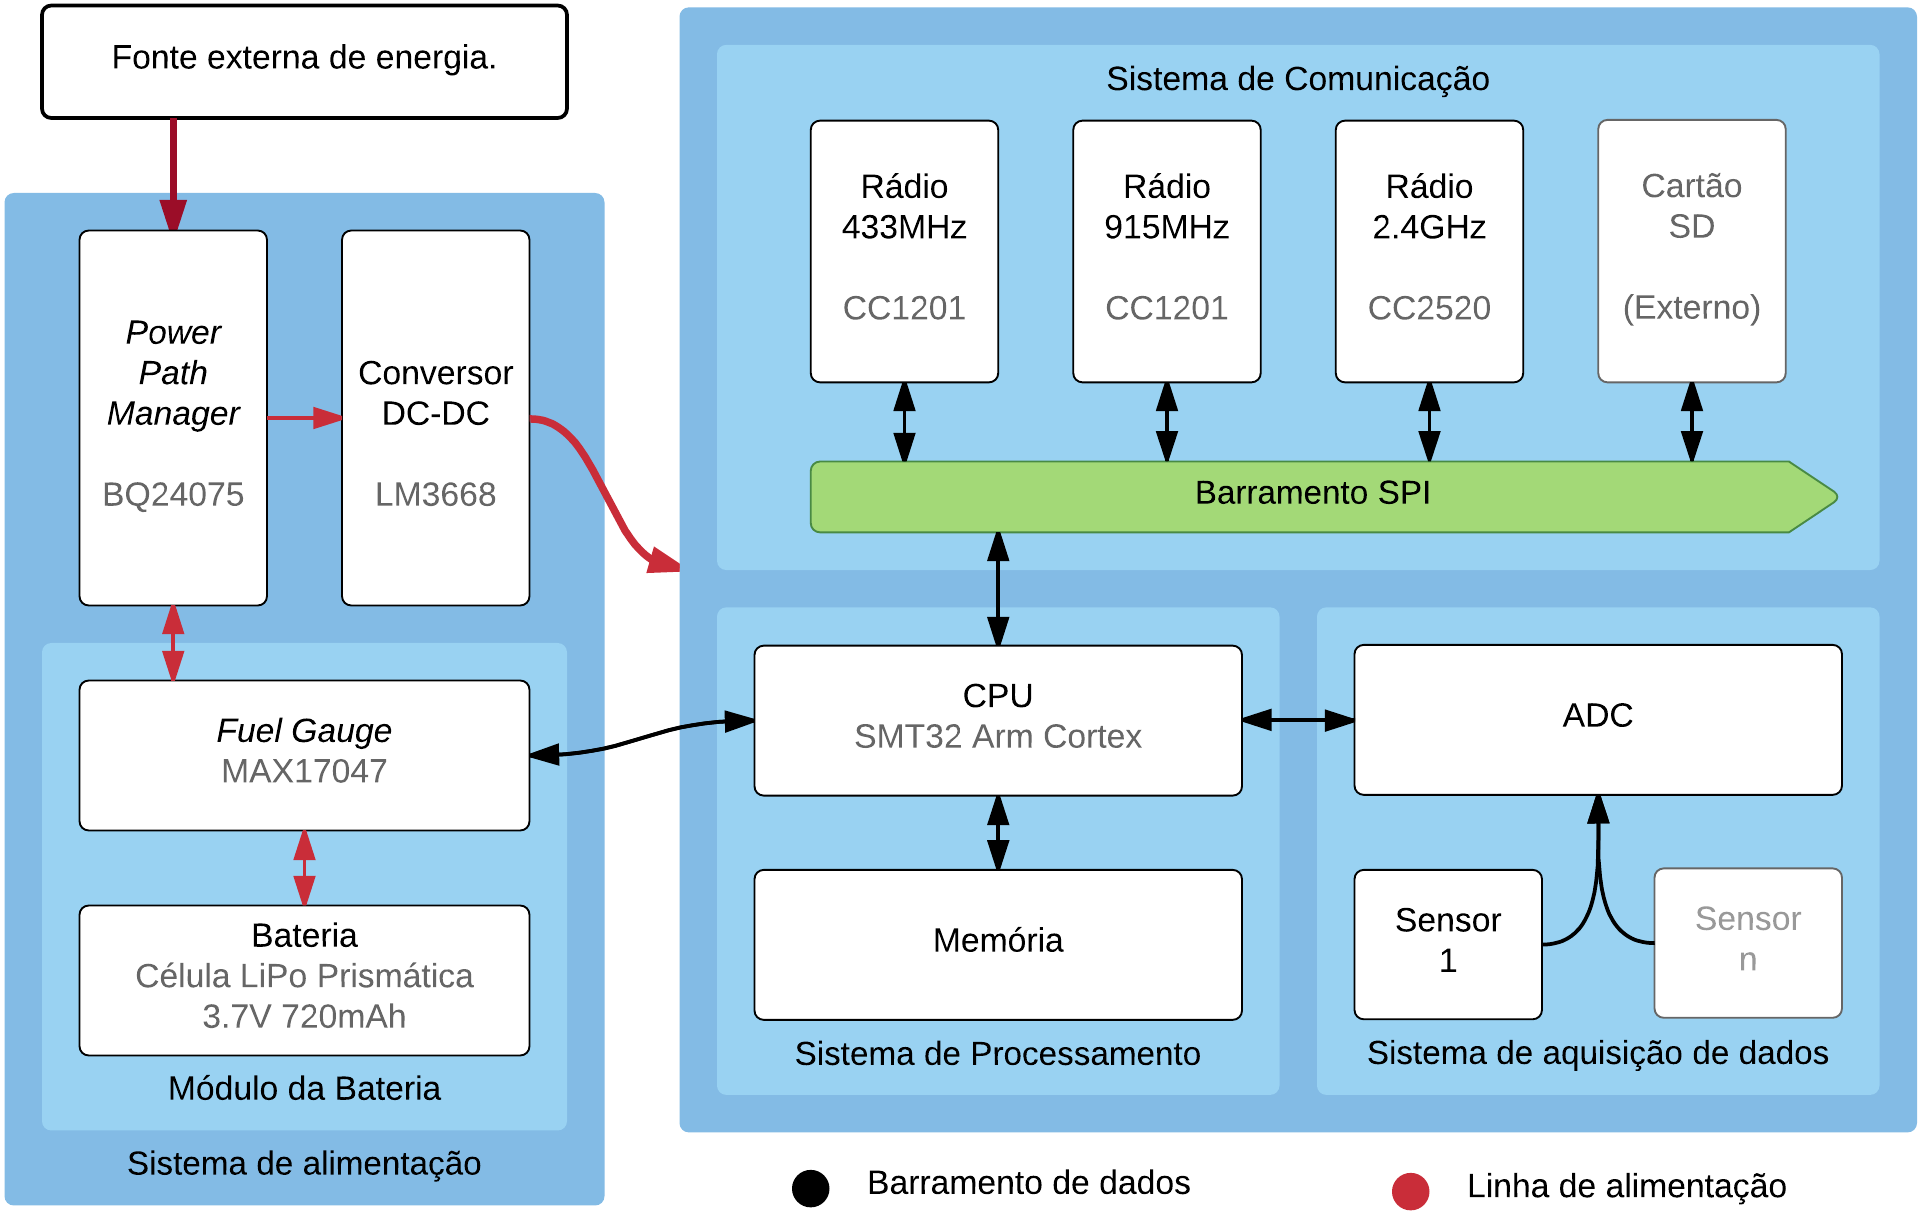
\includegraphics[width=\linewidth]{SensorNode_PhyNode}
	\end{center}
	\legend{Elaboração própria.}
\end{figure}

Com este objetivo introduz-se aqui a plataforma PhyNode. Esta plataforma é composta por dois módulos principais: processamento e sistemas. A \autoref{fig_phynode} ilustra sua arquitetura completa. Esta arquitetura foi baseada no modelo genérico, introduzido na \autoref{fig_node_generic}. No entanto alguns refinamentos, foram acrescentados de forma a atualizá-la com as tecnologias mais atuais, disponíveis no universo da eletrônica embarcada de baixa potência, e equipá-la para realizar os ensaios que serão propostos na segunda etapa deste trabalho.

\subsection{Sistema de processamento}

O módulo de processamento contém o sistema de processamento e a instrumentação necessária para programação e depuração do microcontrolador (MCU). Optou-se para este módulo pela utilização de uma placa de desenvolvimento comercialmente disponível, a STM32Nucleo 64, fabricada pela ST\textsuperscript{\textregistered} Microelectronics. Estas placas contam com uma conexão USB utilizada para programação, depuração e, se necessário, alimentação; possuem ainda interfaces compatíveis com as do Arduino Uno Rev.3\texttrademark, e conectores Morpho\texttrademark ( que disponibilizam acesso a todos os pinos da MCU e às linhas de alimentação disponíveis na placa). Convenientemente são disponibilizados diferentes modelos desta placa, com o mesmo \textit{form-factor}, porém equipadas com diferentes MCUs da linha STM32\texttrademark.

O segundo módulo da plataforma PhyNode, o módulo de sistemas, consiste num \textit{shield}, projetado para encaixar-se diretamente nos conectores Morpho das placas STM32Nucleo 64.

\subsection{Sistemas de alimentação}

Certos refinamentos introduzidos pela plataforma PhyNode encontram-se no módulo de sistemas. A começar pelo sistema de alimentação, uma vez que a eficiência dos demais componentes depende fortemente dele. A seguir serão discutidos dois novos componentes adicionados a este sistemas: o \textit{Power Path Manager} e a \textit{Fuel Gauge}. Posteriormente serão justificadas as escolhas feitas em relação aos demais componentes, e os avanços obtidos com a nova arquitetura serão discutidos.

\begin{itemize}
	\item \textit{Power Path Manager (PPM).} Este componente é responsável por distribuir da maneira mais eficiente possível a energia disponível. Nos protótipos construídos para avaliação da arquitetura proposta, esta funcionalidade é provida pelo chip BQ24075, produzidos pela Texas Instruments\texttrademark. Este chip utiliza o sistema DPPM (\textit{Dynamic Power Path Management}) capaz de alimentar o sistema enquanto simultânea e independentemente carrega a bateria. O algoritmo utilizado pelo DPPM prioriza o fornecimento de energia ao circuito de saída (linhas de alimentação dos demais sistemas). Caso detecte que a voltagem no circuito de entrada (conexão USB, painel solar etc.) começou a cair em decorrência de uma limitação de potência, ele reduz a corrente de carga da bateria. Desta forma é possível priorizar o fornecimento de potência aos demais sistemas, enquanto a corrente de carga da bateria é constantemente calibrada a fim de aproveitar toa a potência disponível no circuito de entrada. Este sistema também permite que a bateria seja utilizada para suplementar a corrente fornecida pelo circuito de entrada durante picos de consumo do sistema. Quando não há uma fonte conectada ao circuito de entrada, a bateria fornece toda a energia consumida \cite{TexasInstruments2014}.
	
	Adicionalmente é interessante ressaltar que o carregamento de bateris de lítio geralmente requer circuitos dedicados e razoavelmente complexos e precisos, a fim de  evitar danos à bateria ou incêndio. O BQ24075 já integra estes circuitos, reduzindo a contagem de componentes total do sistema e economizando algum espaço na superfície da placa de circuito impresso so \textit{shield}.
	\item \textit{Fuel Gauge}. Este componente provê PhyNode com uma nova funcionalidade: monitorar digitalmente, e com precisão, o estado de carga da bateria. Pra esta finalidade a arquitetura proposta utiliza o chip MAX17047, produzido pela Maxim Integrated\texttrademark. Este chip conta com o sistema ModelGauge\texttrademark m3, capaz de monitorar simultaneamente a corrente que circula pela bateria e sua voltagem. Neste sistema, dois algoritmos inteirnamente compensados são utilizados para calcular o estado de carga da bateria. O primeiro deles, conhecido como contador de Coulomb, consiste num circuito integrador que monitora a voltagem e a intensidade da corrente que circula pela bateria ao longo do tempo. Sabendo-se quanta energia fluiu para o interior da bateria,qual a potência consumida ao longo do tempo e, compensando estes valores com coeficientes específicos para a química utilizada na bateria em questão, é possível calcular qual é o seu estado de carga presente.
	
	A Maxim Integrated\texttrademark alega, no entanto, que este sistema, apesar de apresentar resultados mais precisos a curto prazo, apresenta problemas de precisão a longo prazo. Isto se deve, principalmente, às tolerâncias de certos componentes do circuito utilizado para aferição da corrente (mais precisamente um resistor \textit{shunt} que não pode ser integrado ao \textit{chip}, e o traçado das trilhas na placa de circuito impresso). O segundo algoritmo, nomeado ModelGauge\texttrademark, é um algoritmo proprietário desenvolvido pelo fabricante, baseado somente no monitoramento da voltagem da bateria, que é alegadamente mais preciso a longo prazo.
	
	As leituras fornecidas pelo MAX17047 combinam resultados obtidos a partir destes dois algoritmos com fatores de compensação adicionais que dizem respeito a temperatura e ao envelhecimento da bateria. Através deste chip é possível ainda monitorar outros parâmetros do sistema como: consumo instantâneo e o tempo restante para o carregamento ou descarregamento completo da bateria.
	\item \textit{Conversor DC-DC.} O conversor DC-DC desempenha um papel importante para a eficiência energética do sistema. Todo processo de conversão de voltagem ocorre com eficiência inferior a 100\%, indicando que há um custo relacionado à regulação das linhas de alimentação. Porém, mais que isso: quer dizer que este custo é proporcional ao consumo dos sistemas, e que a eficiência de qualquer componente alimentado pelo conversor também é afetada. Em suma, a eficiência global da plataforma depende da escolha de um sistema de conversão adequado.
	
	A utilização de conversores DC-DC é necessária pois as voltagens fornecidas por baterias variam de acordo com seu estado de carga, com a intensidade da corrente consumida e até mesmo de acordo com a temperatura. A maioria dos circuitos de baixa potência atuais, por exemplo, atua na faixa de 3.3 volts. Já as baterias de lítio comumente utilizadas para alimentar os nodos de sensores, podem fornecer voltagens que variam entre 4.2 volts, quando totalmente carregadas, a 2.8 volts em seu estado de carga mais baixo.
	
	O conversor DC-DC selecionado para equipar os protótipos de PhyNode, Texas Instruments LM3668SD-2883, é capaz de manter a regulação de voltagem de saída em 3.3 volts a partir de toda a faixa de voltagem fornecida pela baterias de lítio que equipam os protótipos. Sendo capaz de reduzir eficientemente a voltagem de entrada quando esta se encontrar acima dos 3.3 volts e elevá-la quando encontrar-se abaixo.
\end{itemize}

\subsection{Sistema de comunicação}

O maior diferencial da plataforma PhyNode, no entanto, é seu sistema de comunicação, capaz de operar através de múltiplas interfaces de comunicação simultaneamente. A seguir serão apresentados os componentes utilizados neste sistema e serão discutidos os vanços obtidos e as capacidades dos mesmos.

A começar pela escolha dos rádios: o módulo de sistemas da plataforma PhyNode conta com três radiotransmissores operando em frequências distintas e razoavelmente espaçadas, sendo elas 433MHz, 915MHz e 2.4GHz. A escolha destas frequências foi crucial para o processo de desenvolvimento dos protótipos, uma vez que influencia diretamente em alguns aspectos do seu projeto como, por exemplo, restrições legais para operação e licenciamento de bandas, logística para aquisição de \textit{hardware} e outros. Os principais requisitos estabelecidos foram:

\begin{itemize}
	\item \textit{spalhar o espectro de transmissão tanto quanto possível.} A principal idéia por trás da diversidade de interfaces é implementar dois ou mais links paralelos e independentes, de modo que a probabilidade de todos os links falharem simultaneamente seja pequena. Links independentes podem ser obtidos, por exemplo, utilizando-se faixas de frequência diferentes \cite{Kusy2011}. Quanto maior o espaçamento entre faixas de frequência utilizadas, menor será a dependência entre os links.
	\item \textit{Utilizar apenas bandas ISM.} As faixas de frequência ISM (\textit{Industrial, Scientific and Medical}) são faixas de frequência internacionalmente disponibilizadas para utilização por aplicações industriais, científicas e médicas. Não necessariamente relacionadas a sistemas de telecomunicação. A utilização destas bandas é preferida por não haver grandes restrições legais quanto à irradiação nas mesmas. No entanto, este benefício leva também à sua maior desvantagem, que é a grande probabilidade de sofrer interferências externas, causadas por outros sistemas operando em frequências similares, notadamente redes WiFi e eletrodomésticos como, por exemplo, fornos micro-ondas \cite{Kusy2011, Srinivasan2008}. O espalhamento espectral ajuda a mitigar este problema.
	\item \textit{Não impor grandes restrições à construção física dos nodos.} O projeto de placas de circuito capazes de conduzir adequadamente os sinais de alta frequência é em si um grande desafio. Fatores que antes não importavam como, por exemplo, a geometria das trilhas, sua impedância característica e a espessura da placa, devem ser considerados. Ignora-los significaria incorrer em grandes perdas de eficiência ou até mesmo na completa inutilização dos circuitos de transmissão. AS exigências técnicas para obter-se circuitos eficientes são diretamente proporcionais à frequência. Por este motivo frequência superiores a 2.4GHz foram evitadas.
	\item \textit{Ser compatível com transmissores 802.15.4 eficientes e disponíveis comercialmente.} A eficiência dos links de comunicação depende muito do hardware utilizado. Escolher o transmissor mais adequado é, assim como tantos outros aspectos do projeto de sistemas de hardware e software, uma questão de \textit{co-design} de hardware e software. Porém neste caso limitada pela disponibilidade de produtos comercialmente disponíveis.
\end{itemize}

\begin{table}[bt]
	\centering
	\caption{Comparativo de radiotransmissores}
	\label{tab_transceivers}
	\begin{tabular}{|l|l|l|l|l|l|l|}
		\hline
		\rowcolor[HTML]{C0C0C0} 
		\multicolumn{1}{|c|}{\cellcolor[HTML]{C0C0C0}\textbf{Modelo}} & \multicolumn{1}{c|}{\cellcolor[HTML]{C0C0C0}\textbf{Frequência}} & \multicolumn{1}{c|}{\cellcolor[HTML]{C0C0C0}\textbf{Banda}} & \multicolumn{1}{c|}{\cellcolor[HTML]{C0C0C0}\textbf{Modulação}} & \multicolumn{1}{c|}{\cellcolor[HTML]{C0C0C0}\textbf{TX}} & \multicolumn{1}{c|}{\cellcolor[HTML]{C0C0C0}\textbf{RX}} & \multicolumn{1}{c|}{\cellcolor[HTML]{C0C0C0}\textbf{Potência}} \\ \hline
		CC1000 & 1 $\sim$ 3 GHz & 76.8 Kbps & 2-FSK & 18.5 mA & 9.6 mA & 10 dBm \\ \hline
		nRF903 & 433 / 915 MHz  & 76.8 Kbps & GFSK & 19.5 mA & 22.5 mA & 10 dBm \\ \hline
		TR1000 & 916 MHz & 115.1 Kbps & OOK, ASK & 12.0 mA & 3.8 mA & 0 dBm \\ \hline
		\textbf{CC1201} & ISM Sub 1GHz & 1.25 Mbps & \begin{tabular}[c]{@{}l@{}}2-FSK, 2-GFSK,\\ 4-FSK, 4-GFSK,\\ MSK, OOK\end{tabular} & 46.0 mA\footnote{Corrente de pico para frequência de transmissão 915MHz a +14dBm.} & 8.0 uA\footnote{Corrente média consumida utilizando o sistema eWOR (\textit{enhanced Wake On Radio}) operando a 1Hz.} & 16 dBm \\ \hline
		CC2420 & 2.4 GHz & 250 Kbps & DSSS, O-QPSK & 17.4 mA & 19.7 mA & 0 dBm \\ \hline
		CC2500 & 2.4 GHz & 512 Kbps & 2-FSK & 12.8 mA & 21.6 mA & 1 dBm \\ \hline
		\textbf{CC2520} & 2.4 GHz & 250 Kbps & O-QPSK & 33.6 mA & 18.8 mA & 5 dBm \\ \hline
	\end{tabular}
	\legend{Fonte: Adaptado de \cite{Baccour2012}}
\end{table}

Adicionalmente, num sistema dotado de múltiplas interfaces, o ideal é que o formato dos barramentos de comunicação entre as diversas interfaces e a MCU seja o mais uniforme possível \cite{Lymberopoulos2008}. Devido à grande distância entre as faixas de frequência utilizadas nas três interfaces da plataforma PhyNode não foi possível encontrar um único modelo de transmissor que fosse capaz de lidar com todas elas. No entanto foram escolhidos modelos com arquiteturas compatíveis entre si e equipados com interfaces de comunicação semelhantes.

O CC1201, produzido pela Texas Instruments, é um transmissor de baixa potência, capaz de operar em todas as faixas de frequência ISM Sub 1GHz. Este transmissor conta com avançadas funcionalidades implementadas em hardware, como \textit{engine} criptográfica AES de 128bits, \textit{Clear Channel Assessment} (CCA) e um sistema de \textit{Wake on Radio} (eWOR) que provê baixo consumo no modo de escuta. Este modelo foi selecionado para implementação das interfaces operando nas frequências 433MHz e 915MHz. O CC1201, no entanto, não é capaz de operar na faixa de 2.4GHz, utilizada pela terceira interface. Neste caso foi utilizado outro modelo, o CC2520, também produzido pela Texas Instruments, dotado de funcionalidades semelhantes, porém adicionalmente compatível com o protocolo ZigBee\textsuperscript{\textregistered}. Na \autoref{tab_transceivers}, expandida a partir de dados presentes em \cite{Baccour2012}, encontra-se um comparativo entre os modelos selecionados e alguns outros comumente utilizados.

A fim de prover uma arquitetura modular e expansível para a plataforma PhyNode, os três radiotransmissores são conectados ao mesmo barramento SPI (\textit{Serial Peripheral Interface}) e a MCU dedica uma de suas interfaces de comunicação exclusivamente a este barramento. A conexão de interfaces externas adicionais também é suportada. A comunicação entre os tranmissores e a MCU é incrementada através do uso de pinos de interrupção programáveis. O CC2520 conta com seis destes pinos, e o CC1201 conta com três deles. Já as MCUs permitem que a maioria de seus pinos sejam conectados programaticamente a alguns barramentos internos de interrupção, capazes de operar com diferentes níveis de prioridade. A utilização de pinos de interrupção programáveis possibilita a notificação quase instantânea de diversos eventos, sem que seja necessário para isso utilizar o barramento de comunicação e rotinas de \textit{pooling}, o que viabiliza a implementação de rotinas de tratamento mais eficientes e de menor latência. Este recurso também torna possível que componentes aguardem certos eventos em modo de baixo consumo, sendo acordados através das interrupções quando necessário.

\begin{figure}[hbt]
	\centering
	\caption{\label{fig_prototype}Protótipos do módulo PhyNode}
	\begin{subfigure}{.5\textwidth}
		\centering
		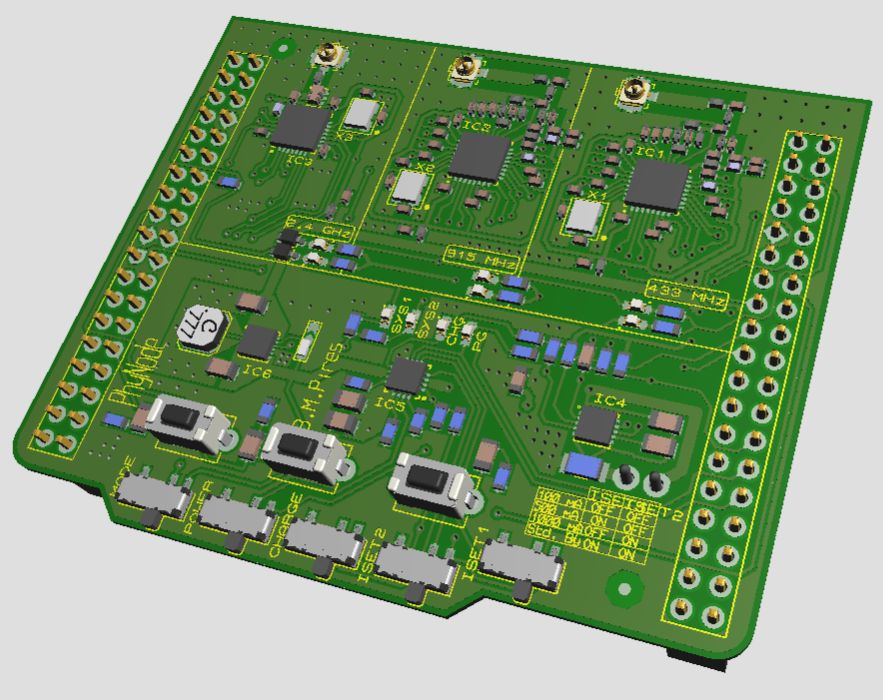
\includegraphics[width=.98\linewidth]{PhyNode_3D}
		\captionsetup{width=.9\textwidth}
		\caption{Simulação 3D da montagem final do módulo PhyNode no software Proteus (CAD)}
		\label{fig_prototype_3d}
	\end{subfigure}%
	\begin{subfigure}{.5\textwidth}
		\centering
		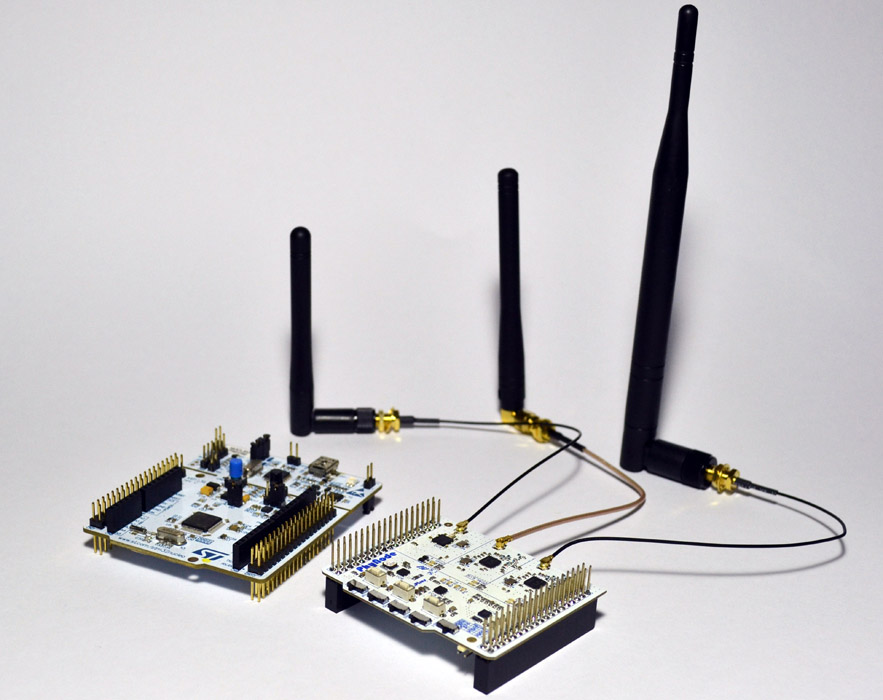
\includegraphics[width=.98\linewidth]{PhyNode_Assembled}
		\captionsetup{width=.9\linewidth}
		\caption{Módulo de comunicação PhyNode, a esquerda. Do lado direito uma Nucleo Board.}
		\label{fig_prototype_assembled}
	\end{subfigure}
	\legend{Fonte: Elaboração própria.}
\end{figure}

A \autoref{fig_prototype_3d} apresenta uma modelagem 3D do \textit{shield} de sistemas da plataforma PhyNode, disponibilizada pelo software CAD utilizado para seu projeto. Pode-se reparar nos três circuitos de transmissão, situados na parte superior do shield. A \autoref{fig_prototype_assembled} apresenta o primeiro protótipo já montado, com as respectivas antenas conectadas, a direta o \textit{shield} de sistemas e a esquerda uma STM32Nucleo.

% ---
% Não editado
% ---

\begin{center}
	\textbf{--- Texto em elaboração - INÍCIO ---}
\end{center}

Dado que a utilização de diferentes modulações, ou bandas de frequência, resulta, de acordo com as condições do ambiente, em alterações na qualidade dos links de rádio \cite{bibid}, considera-se que seja possível explorar a diversificação de interfaces admitida pela norma a fim de otimizar a performance de links de comunicação. No caso de dispositivos dotados de múltiplas interfaces, uma forma através da qual este objetivo pode ser alcançado é utilizando um algoritmo de seleção dinâmica, capaz de eleger a interface mais adequada, a cada momento, para a transferência dos dados. Com este objetivo, nas seções seguintes, será proposta a arquitetura batizada de PhyNode, dotada de três interfaces IEEE 802.15.4, operando nas bandas de frequência de 433 MHz, 915 MHz e 2450 MHz. Selecionadas a fim de satisfazer as exigências da regulamentação local, de acordo com a resolução nº 452 da ANATEL \cite{bibid} e a fim de prover a maior amplitude espectral possível.

% ---

A plataforma PhyNode inclui três \textit{transceivers}, sendo dois CC1201 \cite{bibid} destinados às bandas de frequência sub-GHz e um CC2520 \cite{bibid}, destinado à banda de 2450 MHz. As configurações disponíveis em cada um destes componentes permitem que, em alguns casos, mais de um PHY seja utilizado através do mesmo \textit{transceiver}, porém  não simultaneamente.
	\section{Diversidade de Interfaces}
	PhyNode pode utilizar-se do identificador único de 32bits presente no padrão IEEE 802.15.4 para carregar as configurações adequadas num \textit{trasnceiver} antes de transmitir um pacote de dados. O conjunto de PHYs IEEE 802.15.4 suportados em PhyNode é apresentado na Tabela \ref{tab:modos_opr}.
	
	\begin{table}[h]
		\centering
		\begin{tabular}{|c|c|l|l|l|l|l|}
			\hline
			\textbf{Página}    & \multicolumn{1}{l|}{\textbf{Canais}}   & \textbf{Banda}          & \textbf{Modulação}   & \textbf{Taxa transf.} \\ \hline
			0                  & 11$\sim$26                             & 2450MHz                 & O-QPSK               & 250Kb/s               \\ \hline
			1                  & 1$\sim$10                              & 915MHz                  & ASK                  & 250Kb/s               \\ \hline
			\multirow{3}{*}{7} & \multirow{3}{*}{0$\sim$14}             & \multirow{3}{*}{433MHz} & \multirow{3}{*}{MSK} & 250Kb/s               \\
			&                                        &                         &                      & 100Kb/s               \\
			&                                        &                         &                      & 31.25Kb/s             \\ \hline
			9                  & 0$\sim$128                             & 915MHz                  & 2-FSK                & 50Kb/s                \\ \hline 
		\end{tabular}
		\caption{Modos de operação suportados}
		\label{tab:modos_opr}
	\end{table}
	
	As frequências dos canais disponíveis especificamente nos PHYs utilizados pelos módulos PhyNode são  descritas de acordo com as equações (\ref{eq:ch433msk}), (\ref{eq:ch915ask}), (\ref{eq:ch915fsk}) e (\ref{eq:ch2450oqpsk}).
	
	\begin{equation}
	\label{eq:ch433msk}
	f_{P0}(C) = 433.164 + 0.108\times C, \forall C \in \{0..14\}
	\end{equation}
	
	\begin{equation}
	\label{eq:ch915ask}
	f_{P1}(C) = 906 + 2 (C - 1), \forall C \in \{1..10\}
	\end{equation}
	
	\begin{equation}
	\label{eq:ch915fsk}
	f_{P7}(C) = 902.2 + 0.2 \times C, \forall C \in \{0..128\}
	\end{equation}
	
	\begin{equation}
	\label{eq:ch2450oqpsk}
	f_{P9}(C) = 2405 + 5 (C - 11), \forall C \in \{11..26\}
	\end{equation}
	
	Adicionalmente é possível selecionar a potência de transmissão utilizada por cada \textit{trasnceiver}, sendo que o modelo CC1201 é capaz de operar entre -40 DBm e 14 DBm (ou -37 DBm a 17 DBm, considerando-se o uso de antenas com ganho de 3 DBi), já o modelo CC2520 pode operar entre -18 DBm e 5 DBm (ou -13 DBm a 10DBm, considerando-se o uso de antenas com ganho de 5 DBi).
	
	Também é importante ressaltar que para que se possa estabelecer um link entre dois dispositivos eles devem estar alinhados quanto à diversos parâmetros, com exceção geralmente apenas da potência de transmissão. Para que estes parâmetros possam ser alterados dinamicamente é são requeridos mecanismos de sincronia, responsáveis manter ambas as configurações atualizadas em ambas as extremidades do link.
	\section{Parâmetros observáveis}
	CC2520
	\begin{itemize}
		\item EIRP = -13 ~ 10
		\item CHANNEL = 2405 ~2505 [16]
	\end{itemize}
	CC1201
	\begin{itemize}
		\item EIRP = -37 ~ 17
		\item CHANNEL = 410 ~ 475 [14]
		\item SYMBOL RATE
		\item MODULATION
	\end{itemize}
	Common
	\begin{itemize}
		\item Packet length
		\item Packet interval
	\end{itemize}
	Output parameters
	\begin{itemize}
		\item RSSI
		\item LQI
		\item CRC\_OK
	\end{itemize}
	
\begin{center}
	\textbf{--- Texto em elaboração - FIM ---}
\end{center}
	
\section{Caracterização dos links}

\begin{center}
	\textbf{--- Seção em elaboração ---}
\end{center}

\chapter{PhyMAC: Camada MAC multi-interface} \label{phymac}
% TODO PhyMAC

\begin{center}
	\textbf{--- Seção em elaboração ---}
\end{center}

% ---
% Resultados
% ---
\chapter{Avaliação experimental}
% TODO Avaliação experimental

\begin{center}
	\textbf{--- Seção em elaboração ---}
\end{center}

% ----------------------------------------------------------
% Finaliza a parte no bookmark do PDF
% para que se inicie o bookmark na raiz
% e adiciona espaço de parte no Sumário
% ----------------------------------------------------------
\phantompart

% ---
% Conclusão
% ---
\chapter{Conclusão}
% TODO - Conclusão

\begin{center}
	\textbf{--- Seção em elaboração ---}
\end{center}

% ----------------------------------------------------------
% ELEMENTOS PÓS-TEXTUAIS
% ----------------------------------------------------------
\postextual
% ----------------------------------------------------------

% ----------------------------------------------------------
% Referências bibliográficas
% ----------------------------------------------------------
\bibliography{dissert}

% ----------------------------------------------------------
% Glossário
% ----------------------------------------------------------
%
% Consulte o manual da classe abntex2 para orientações sobre o glossário.
%
%\glossary

% ----------------------------------------------------------
% Apêndices
% ----------------------------------------------------------

% ---
% Inicia os apêndices
% ---
%\begin{apendicesenv}

% Imprime uma página indicando o início dos apêndices
%\partapendices

% ----------------------------------------------------------
%\chapter{Quisque libero justo}
% ----------------------------------------------------------

%\lipsum[50]

%\end{apendicesenv}
% ---


% ----------------------------------------------------------
% Anexos
% ----------------------------------------------------------

% ---
% Inicia os anexos
% ---
%\begin{anexosenv}

% Imprime uma página indicando o início dos anexos
%\partanexos

% ---
%\chapter{Morbi ultrices rutrum lorem.}
% ---
%\lipsum[30]

%\end{anexosenv}

%---------------------------------------------------------------------
% INDICE REMISSIVO
%---------------------------------------------------------------------
\phantompart
\printindex
%---------------------------------------------------------------------

\end{document}
